\documentclass[12pt]{article}
\usepackage[english]{babel}
\usepackage[utf8]{inputenc}
\usepackage{amsmath}
\usepackage{amssymb}
\usepackage{amsthm}
\usepackage{hyperref}
\usepackage{graphicx}
\usepackage{subcaption}
\usepackage{xcolor}
\usepackage{algorithm}
\usepackage{algpseudocode}
\usepackage{parskip}

\graphicspath{{figures/}}

\newcommand{\todo}[1]{\textcolor{red}{#1}}

\newcommand{\R}{\mathbb{R}}
\newcommand{\N}{\mathbb{N}}

\newcommand{\loc}{x}
\newcommand{\tim}{t}
\newcommand{\ind}{i}
\newcommand{\data}{d}
\newcommand{\traj}{r}
\newcommand{\cotraj}{\mathcal{R}}
\newcommand{\pred}{p}
\newcommand{\swap}{s}
\newcommand{\swaptime}{u}
\newcommand{\preswap}{p}

\newcommand{\locset}{\mathbb{L}}
\newcommand{\timeset}{\mathbb{R}_+}
\newcommand{\indset}{\mathbb{N}}
\newcommand{\dataset}{\mathcal{D}}
\newcommand{\trajset}{\mathcal{T}}
\newcommand{\cotrajset}{\mathcal{R}}

\newcommand{\locint}{\mathbf{x}}
\newcommand{\timint}{\mathbf{t}}

\newcommand{\DAG}{G}
\newcommand{\paths}{P}

\newcommand{\graph}{G}
\newcommand{\swapgraph}{G_s}

\newcommand{\locrand}{X}
\newcommand{\trajrand}{R}

\newtheorem{thm}{Theorem}
\newtheorem{proposition}{Proposition}
\newtheorem{lemma}{Lemma}
\newtheorem{example}{Example}

\theoremstyle{definition}
\newtheorem{definition}{Definition}[section]

\title{Privacy and Analysis of Trajectories and Co-Trajectories}
\author{Joel Dahne}

\begin{document}
\maketitle

\tableofcontents

\begin{abstract}
  A trajectory of an individual or object corresponds to its movement
  in space as a function of time. A co-trajectory is a collection of
  trajectories belonging to different individuals or objects. The
  thesis is divided into two parts about two different topics related
  to co-trajectories. The first part is about privacy-preservation in
  co-trajectories and introduces an algorithm called \emph{SwapMob}
  for improving the privacy when handling co-trajectories. In the
  second part we consider different stochastic models for trajectories
  and co-trajectories that is an important tool when analyzing data
  from co-trajectories and using it to make predictions.
\end{abstract}

\section{Introduction}
With today's use of mobile phones and other location aware devices,
such as GPS's, huge amounts of location based data is produced and
used. This enables many new applications that can help both the
individual and the crowd. For the individual this enables the use of
many different location based services, for example navigation
services (such as Google Maps or public transport applications),
social games and networks (such as Pokemon GO) and services for
finding interesting nearby places (such as Yelp). By aggregating data
from multiple people it can also be used for large scale decision
making, for example in city planning it can be used to find commuting
patterns which is helpful for improving public transport and general
infrastructure \cite{novak_application_2013,
  pinelli_data-driven_2016}.

Both of these use cases come with privacy concerns. Mobility data
contains a lot of potentially sensitive information, among other
things it can contain data about visits to hospitals and religious
places along with time spent at home or at work. For location based
services the individual wants the utility from the service but also
privacy. If the service provider knows who you are, often the case
with for example Googles services, then giving them access to your
mobility data allow them to combine this with other data to learn more
about you. Other times you are communicating with the service provider
under a pseudonym, many public transport application works like this,
in which case you are not directly linked to the data. However, due to
the high degree of uniqueness of mobility data re-identification of
the individual is still often possible \cite{de_montjoye_unique_2013}.
Because of this a balance between privacy and utility when using
location based data has to be found.

The focus of this thesis is on the usage of aggregated location data.
We begin by giving a mathematical definition of trajectories and
co-trajectories. After that the thesis is divided into two parts, one
about privacy and one about stochastic models for co-trajectories. The
privacy part begins with a brief introduction about previous work on
the topic. Then we take a look at one method, SwapMob, useful for
improving privacy when working with co-trajectories, which was
introduced in the literature last year. We give a more formal
definition of the method than previously done and analyse its
properties. For the part about stochastic models we first present a
very general model for co-trajectories. Then we look closer at a more
specific Markov chain model.

\section{Trajectories and co-trajectories}
\label{sec:traj-and-co-traj}
In this section we introduce and define trajectories and
co-trajectories. We begin by, informally, explaining the meaning we
associate with a trajectory and a co-trajectory and then continue by
giving a formal definition.

A trajectory is given by the movement of an object, for example, a
person or a bus, and can be seen as a function of time giving the
location of the object at the time. For example we can consider the
trajectory of a person on their way to work, or that of an airplane
flying between two airports. Both of these examples are naturally
continuous, the location changes continuously with time. We can
consider trajectories which are discontinuous as well, for example the
location of a persons home, which stays constant most of the time and
then jumps to another place whenever the person moves.

When considering a number of trajectories together, each associated
with a different object, we are talking about a collection of
trajectories, a co-trajectory. A co-trajectory could for example be
the trajectories of all, or some, buses in a city for a given day, or
the trajectories of all airplanes leaving an airport. We can also have
less homogeneous co-trajectories, such as a co-trajectory consisting
of trajectories for the commuters in a city together with the
trajectories of the buses.

When considering how to define a trajectory we have to take into
account that the true movement of an object is in general not known.
Most trajectories are naturally continuous, but we cannot capture or
measure the continuous movement of the trajectory in practice.
Typically, the location of an object at some time is given by a
discrete measurement of its current location up to some precision. We
therefore adopt a definition of a trajectory which is more related to
how we get information about the movement of an object in practice,
discrete measurements of its location in space and time.

Performing a measurement gives a datapoint, a datapoint is given by a
time and a location for the object. How the location is given depends
on what is being measured; for a car it could be given by GPS
coordinates or the location on a map, for an airplane you could have
GPS coordinates together with an altitude. We can also consider cases
when the location is discrete and without an explicit representation
in space, such as an address or a node in a graph that represents the
road network for instance. In general we use the notation \(\locset\)
for the set of locations, depending on the application different
choices for \(\locset\) can then be used.
\begin{definition}[\textbf{Datapoint}]
  \label{def:datapoint}
  A datapoint, \(\data\), is given by
  \(\data = (\loc, \tim) \in \locset \times \timeset\) giving the the
  location, \(\loc\), and the time, \(\tim\), for the datapoint. The
  set of all datapoints, \(\locset \times \timeset\), will be denoted
  by \(\dataset\).
\end{definition}
For a datapoint \(\data\) we refer to \(\loc\) as the location of the
datapoint and \(\tim\) as the time or the timestamp of it.

A trajectory is now given by a set of datapoints with no two
datapoints sharing the same time. We do allow for an infinite number
of datapoints but will require that in every finite time interval
there is only a finite number of them. In practical applications the
number of datapoints will of course be finite, but this is relevant
when discussing stochastic models for trajectories in Section
\ref{sec:modell-co-traj}.
\begin{definition}[\textbf{Trajectory}]
  \label{def:trajectory}
  A trajectory, \(\traj\), is given by a set of datapoints,
  \(\traj \subset \dataset\), satisfying that no two datapoints have
  the same time and that for every finite interval of time there is
  only a finite number of datapoints with the time occurring in this
  interval. We denote the set of all trajectories by \(\trajset\).
\end{definition}
Not allowing datapoints occurring at the same time is reasonable since
an object can in general not be in two places at the same time.
However since in practice the time for the datapoint is necessarily
discretized it could happen that we have two datapoints that are
captured at slightly different times but get the same discretized
timestamp. The main problem with allowing datapoints with the same
timestamp is that there is no natural ordering of the datapoints, we
cannot order them just by their timestamp. If there is a particular
application where multiple datapoints with the same timestamp could
occur then you would have to choose one of them to use, how this is
done will then depend on the application. See Figure
\ref{fig:trajectory} for two examples of trajectories.

\begin{figure}
  \centering
  \begin{subfigure}[t]{0.45\textwidth}
    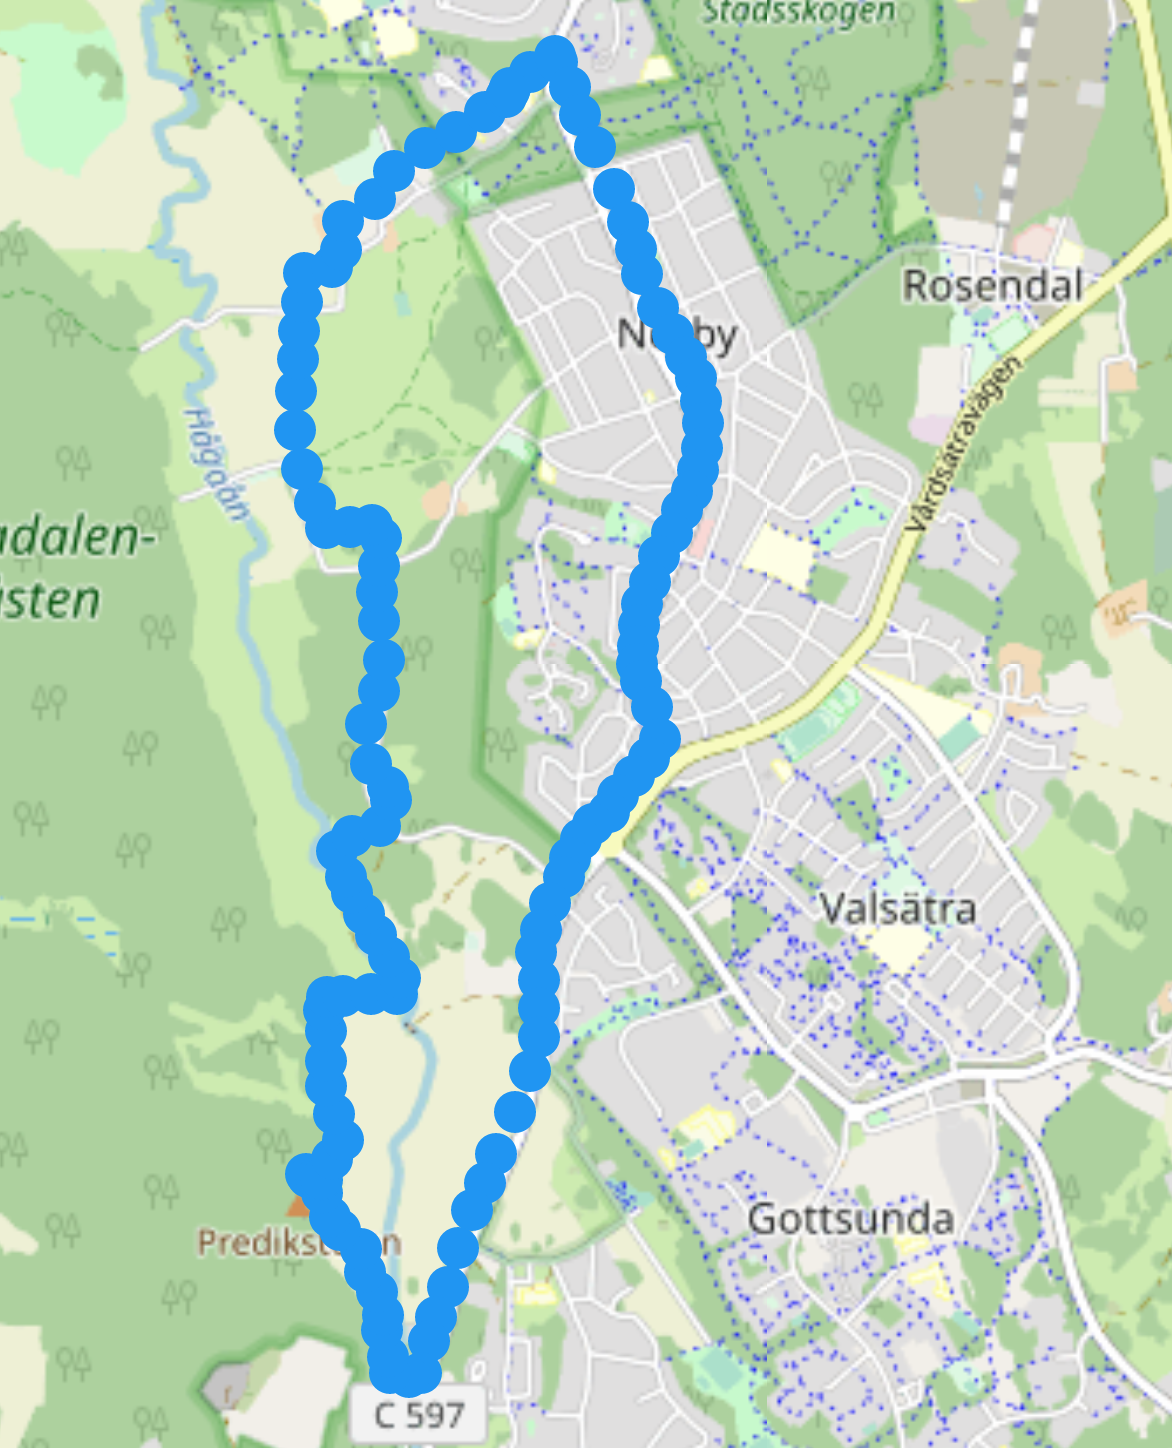
\includegraphics[width=\textwidth]{figures/trajectory-uppsala.png}
    \caption{Trajectory from a person cycling nearby Uppsala.
      \(\locset\) is here given by positions on Earth, in this case
      recorded as longitude and latitude.}
    \label{fig:trajectory-uppsala}
  \end{subfigure}
  \begin{subfigure}[t]{0.45\textwidth}
    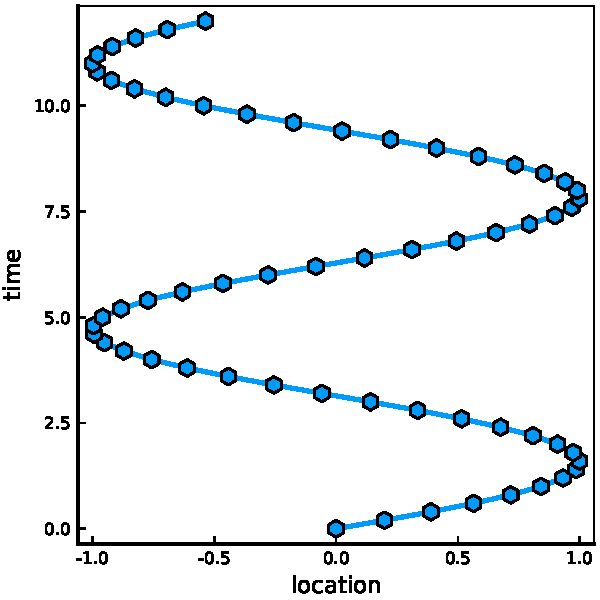
\includegraphics[width=\textwidth]{figures/trajectory_tempospatial.pdf}
    \caption{Trajectory with \(\locset = \R\) with 60 datapoints in
      the time interval \([0, 12]\) where the location for the
      datapoint at time \(\tim\) is given by \(\sin(\tim)\).}
    \label{fig:trajectory-tempospatial}
  \end{subfigure}
  \caption{Two different kinds of trajectories, one based on real
    world data and one on generated data.}
  \label{fig:trajectory}
\end{figure}

A co-trajectory is a collection of trajectories. We allow multiple
occurrences of the same trajectory (this would correspond to different
individuals with the same trajectory) and it is therefore given by a
multiset of trajectories. In our case we are only interested in
co-trajectories with a finite number of trajectories but the
definition could easily be generalized to infinite ones.
\begin{definition}[\textbf{Co-trajectory}]
  \label{def:co-trajectory}
  A co-trajectory, \(\cotraj\), consisting of \(N\) trajectories is
  given by a multiset \(\{\traj_{i}\}_{i = 1}^{N}\) of trajectories
  \(\traj_{i} \in \trajset\).
\end{definition}
Two examples of co-trajectories are given in Figure
\ref{fig:co-trajectory}.

\begin{figure}
  \centering
  \begin{subfigure}[t]{0.49\textwidth}
    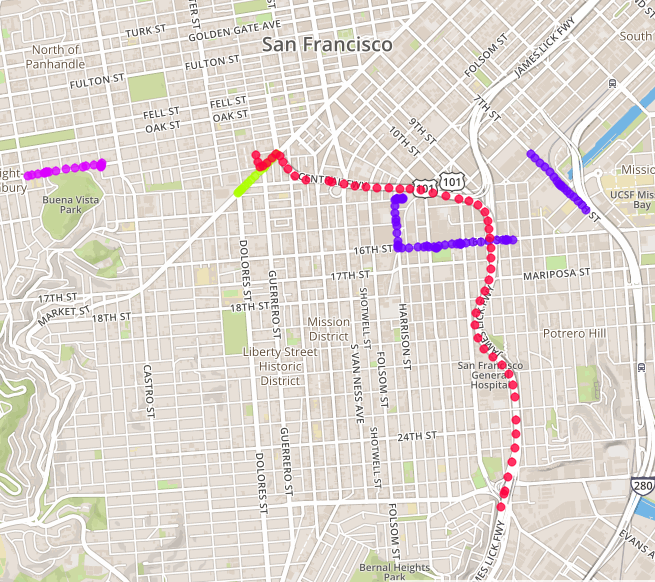
\includegraphics[width=\textwidth]{figures/cotrajectory-taxi.png}
    \caption{A co-trajectory where the trajectories are given by taxi
      rides in San Francisco.}
    \label{fig:co-trajectory-taxi}
  \end{subfigure}
  \begin{subfigure}[t]{0.49\textwidth}
    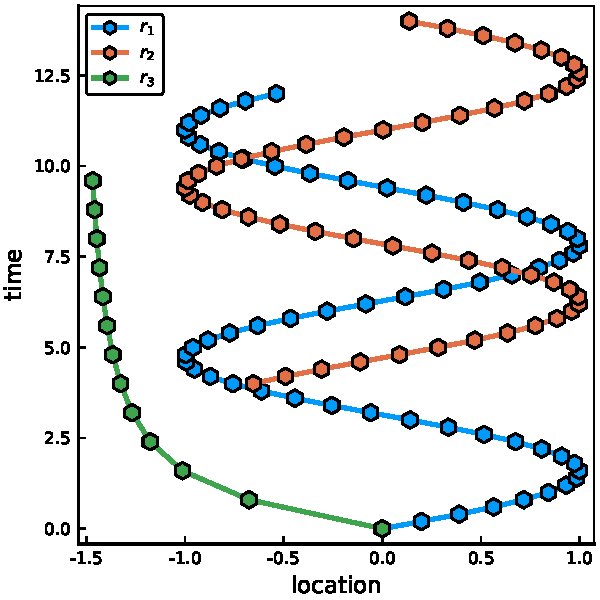
\includegraphics[width=\textwidth]{figures/cotrajectory_tempospatial.pdf}
    \caption{A co-trajectory with \(\locset = \R\) consisting of three
      trajectories, \(\cotraj = \{\traj_{1}, \traj_{2}, \traj_{3}\}\).}
    \label{fig:co-trajectory-tempospatial}
  \end{subfigure}
  \caption{Two different kinds of co-trajectories, one based on real
    world data and one on generated data.}
  \label{fig:co-trajectory}
\end{figure}


\section{Privacy for co-trajectories}
\label{sec:priv-co-traj}
Co-trajectories can, in particular when the individual trajectories
corresponds to people, contain a lot of sensitive data. It can reveal
information about home and work place as well as information about
visits to for example hospitals or religious places
\cite{gambs_show_2010}. Even if the data is anonymized information can
be leaked by for example connecting trajectories with people living at
a certain address. For this reason it is important to take into
account privacy when analysing and publishing data from
co-trajectories \cite{taylor_no_2016}.

A survey of the current state regarding privacy concerns related to
location data is given by Primault et al.~\cite{primault_long_2018}.
They discuss several different privacy threats coming from location
data, these include \emph{Mobility Prediction}, \emph{Social
  Relationships}, \emph{Points of Interests} and
\emph{Re-identification}. Our focus will be on Re-identification, how
an individual can be associated with a trajectory in a co-trajectory.

\subsection{Re-identification for co-trajectories}
\label{sec:re-identification-co}
Re-identification is in general possible due to the high degree of
uniqueness for trajectories of individuals. For example, de Montjoye
et al. \cite{de_montjoye_unique_2013} studied the uniqueness of
mobility data for humans. They had data for one and a half million
individuals given by location of mobile phones as determined by the
carrier's antennas. In the study they conclude that knowledge of four
datapoints for an individual were enough to uniquely identify 95\% of
the population. Very little information is thus needed to identify an
individual even among a very large number of people.

In general re-identification of an individuals trajectory in a
co-trajectory is done using partial data of the trajectory, in the
above study this partial data were four datapoints from the
trajectory. However, partial data about an individuals trajectory
could come in many forms. It could be that we know some of the
datapoints for the trajectory, or we know that the individual
visited some specific area at a certain time. But it could also be
less concrete things, such as knowing that the individual always takes
a specific way when traveling between two places or that the
individual visits the hospital at least once a week.

Since partial data about trajectories could come in many different
forms we need a way to represent and model it to analyze it. To
represent all of these different kinds of partial data we use a
predicate on trajectories. A predicate, \(\pred\), corresponding to
some partial data is a function that given a trajectory returns true
if it satisfies the partial data and false otherwise.
\begin{equation*}
  \pred(\traj) =
  \begin{cases}
    true & \text{ if } \traj \text{ satisfies the partial data,}\\
    false & \text{ otherwise.}
  \end{cases}
\end{equation*}
For example, if we know one datapoint, \(\data\), for the trajectory
we get the predicate \(\pred_{\data}\) that would return true only for
trajectories having this datapoint.
\begin{equation*}
  \pred_{\data}(\traj) =
  \begin{cases}
    true & \text{ if } \data \in \traj\\
    false & \text{ otherwise.}
  \end{cases}
\end{equation*}
If we know that the individual visits the hospital at least once per
week the predicate would return true only for trajectories doing that.

\subsection{Measuring privacy}
\label{sec:measuring-privacy}
To discuss privacy related to co-trajectories we need a way to measure
it. The literature contains many different ways for measuring privacy.
One of the simplest, but still well used, methods is \(k\)-anonymity
introduced by Sweeney \cite{sweeney_k-anonymity:_2002}. A dataset
satisfies \(k\)-anonymity if the information for each individual
cannot be distinguished from at least \(k - 1\) other individuals.

The original definition of \(k\)-anonymity by Sweeney is suitable for
tabular data. Attempts have been made to make it more suitable for
trajectories and one version is \((k, \delta)\)-anonymity introduced
by Abul et al. \cite{abul_never_2008} which considers the imprecision
when measuring location as one part of the anonymity. We take a
slightly different approach and adapt it to our definition of
predicates on co-trajectories. A co-trajectory satisfies
\(k\)-anonymity with respect to a predicate \(\pred\) if at least
\(k\) trajectories satisfy the predicate. If we for a predicate
\(\pred\) denote by \(\pred(\cotraj)\) the set of trajectories in
\(\cotraj\) satisfying the predicate, then it satisfies
\(k\)-anonymity if \(|\pred(\cotraj)| \geq k\). An individual is
uniquely identifiable with respect to a predicate \(\pred\) if
\(|\pred(\cotraj)| = 1\).

This can also be generalized to families of predicates. Given a family
\(\{\pred_{i}\}_{i \in I}\) of predicates a co-trajectory satisfies
\(k\)-anonymity with respect to this family if
\(\min_{i \in I}\pred_{i}(\cotraj) \geq k\).

One limitation of \(k\)-anonymity is that even though the individual
is only one in a group of at least \(k\) it could be that all these
individuals share a specific, possibly sensitive, trait. To handle
this problem Machanavajjhala et al. introduced \(l\)-diversity
\cite{machanavajjhala_l-diversity:_2006}. Simply put it extends
\(k\)-anonymity by also requiring that all groups are sufficiently
diverse. They give a formal definition of when a dataset satisfies
\(l\)-diversity, however their definition is suited to tabular data
that they are working with and less suited for co-trajectories. We do
not aim to give a formal definition of \(l\)-diversity for
co-trajectories but will instead keep the discussions regarding
diversity on an informal level. A co-trajectory has high diversity
with respect to a predicate \(\pred\) if the trajectories in
\(\pred(\cotraj)\) are diverse, i.e. are not to similar to each other.

Both \(k\)-anonymity and \(l\)-diversity will come up when analysing
the privacy of SwapMob in Section \ref{sec:swapmob-analysis}.

\section{SwapMob}
\label{sec:swapmob}
To help protecting the privacy of individuals when working with
location based data many methods have been proposed in the literature.
The goal is to improve the privacy while still being able to use the
data for analysis. The methods vary both in the situation they are
adapted to and the technique used for protecting the privacy. Some of
the methods can be applied to protect privacy for a trajectory from a
single individual, these include data perturbation techniques (e.g.
\cite{andres_geo-indistinguishability:_2013, ghinita_prive:_2007,
  jiang_publishing_2013}) and fake data generation techniques (e.g.
\cite{quercia_spotme_2011, pelekis_privacy-aware_2011,
  kido_protection_2005}). Others are suited for protecting the privacy
of trajectories as one of many in a co-trajectory, e.g. mix-zones
\cite{beresford_location_2003, beresford_mix_2004}.

One recently proposed method for protecting privacy for
co-trajectories is \emph{SwapMob} \cite{salas_swapmob:_2018}. The idea
of SwapMob is to modify the co-trajectory by swapping segments of
trajectories that cross. The goal is to make re-identification of
individuals harder, but still keep enough information to allow the
co-trajectory to be used for analysis. The aim of this chapter is to
give a slightly different, more mathematical, definition of the method
as well as perform a more thorough analysis of the method than done in
the original presentation.

\subsection{Definition}
We begin by defining what we mean by swapping of trajectories, then
continue by defining swapping on co-trajectories and give an
algorithmic description of SwapMob.

Let \(\traj_{1}\) and \(\traj_{2}\) be two trajectories. Swapping
\(\traj_{1}\) and \(\traj_{2}\) refers to moving datapoints between
the two trajectories. More precisely, swapping \(\traj_{1}\) and
\(\traj_{2}\) at time \(\swaptime\) gives us two new trajectories
\(\overline{\traj}_{1}\) and \(\overline{\traj}_{2}\) given by
\begin{equation*}
  \overline{\traj}_{1} = \{(\loc, \tim) \in \traj_{1}: \tim < \swaptime\}
  \cup \{(\loc, \tim) \in \traj_{2}: \tim \geq \swaptime\}
\end{equation*}
and
\begin{equation*}
  \overline{\traj}_{2} = \{(\loc, \tim) \in \traj_{2}: \tim < \swaptime\}
  \cup \{(\loc, \tim) \in \traj_{1}: \tim \geq \swaptime\}.
\end{equation*}
So \(\overline{\traj}_{1}\) consists of the datapoints of
\(\traj_{1}\) before time \(\swaptime\) and the ones of \(\traj_{2}\)
after time \(\swaptime\), and reversed for \(\overline{\traj}_{2}\).
Figure \ref{fig:swapping-spatial} and \ref{fig:swapping-tempo-spatial}
show examples of two trajectories before and after swapping.

\begin{figure}
  \centering
  \begin{subfigure}[t]{0.4\textwidth}
    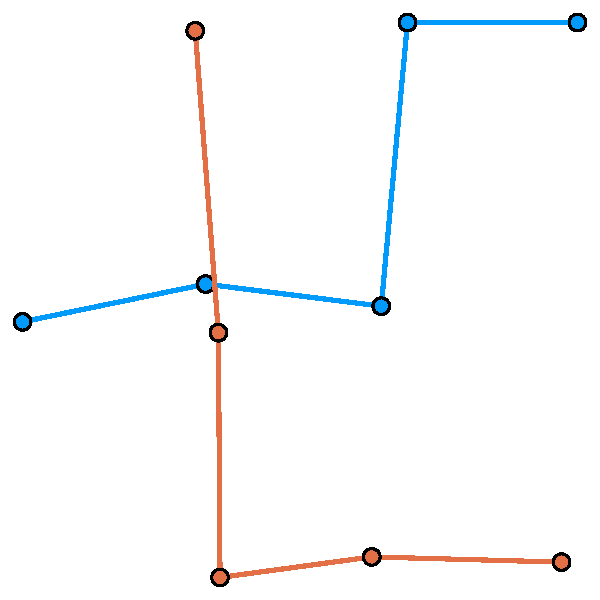
\includegraphics[width=\textwidth]{swapping_spatial-a.pdf}
    \caption{}
  \end{subfigure}
  \begin{subfigure}[t]{0.4\textwidth}
    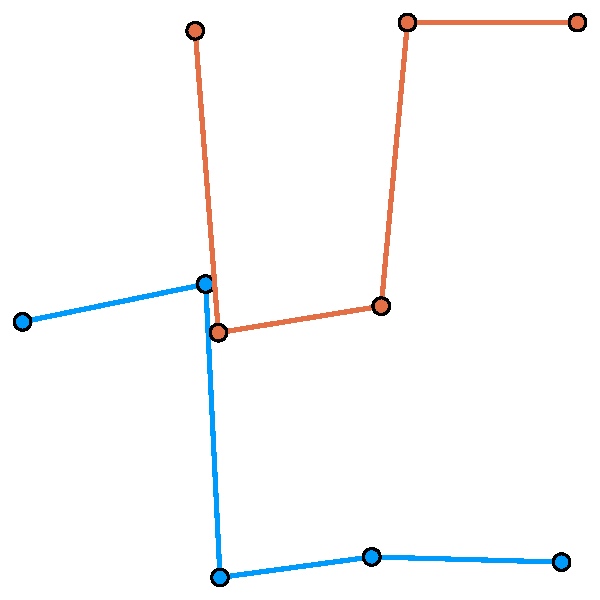
\includegraphics[width=\textwidth]{swapping_spatial-b.pdf}
    \caption{}
  \end{subfigure}
  \caption{Two trajectories with \(\locset = \R^{2}\) are shown before
    swapping, to the left, and after swapping, to the right. The time
    of the datapoints is not explicit in this figure.}
  \label{fig:swapping-spatial}
\end{figure}

\begin{figure}
  \centering
  \begin{subfigure}[t]{0.4\textwidth}
    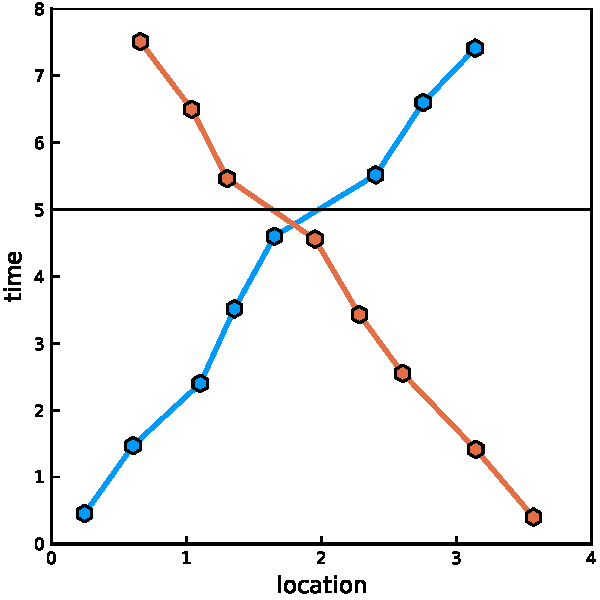
\includegraphics[width=\textwidth]{swapping_tempospatial-a.pdf}
    \caption{}
  \end{subfigure}
  \begin{subfigure}[t]{0.4\textwidth}
    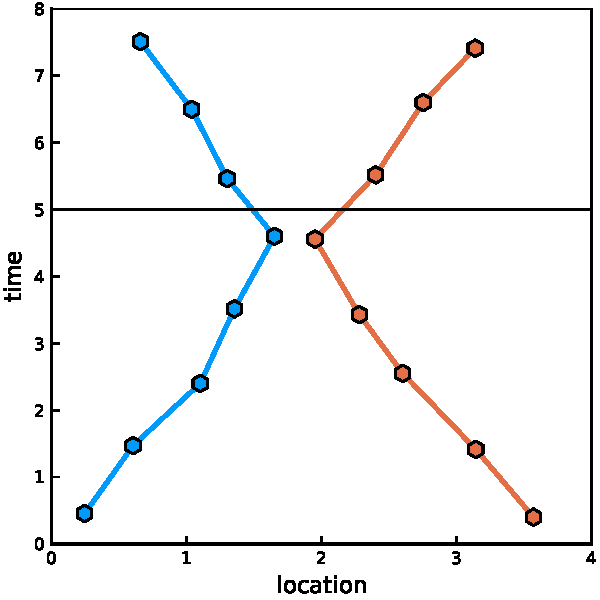
\includegraphics[width=\textwidth]{swapping_tempospatial-b.pdf}
    \caption{}
  \end{subfigure}
  \caption{A trajectories with \(\locset = \R\) is shown before
    swapping in (a) and after swapping in (b). In this figure the
    time is explicit and follows the \(y\)-axis. The swap occurs at
    \(\swaptime = 5\) which is shown by the black line.}
  \label{fig:swapping-tempo-spatial}
\end{figure}


While we can swap two trajectories at any time this will in general
give us trajectories with big jumps in. Consider for example the case
of two trajectories corresponding to two individuals moving in
different parts of a city, swapping their trajectories at some time
would given two trajectories that at that time suddenly jump from one
part of the city the another. To avoid the problem of sudden jumps we
restrict swapping to times when the two trajectories are close to each
other. This is formalized by defining a \emph{similarity} relation for
datapoints. We want two datapoints, \(\data_{1}\) and \(\data_{2}\),
to be similar, denoted by \(\data_{1} \approx \data_{2}\), if they are
close in both space and time. If \(\locset\) is a metric space one
definition is to let \(\data_{1} \approx \data_{2}\) if the distance
between them in both space and time is below some given threshold. The
big drawback of this approach is that it is not an equivalence
relation, i.e. \(\data_{1} \approx \data_{2}\) and
\(\data_{2} \approx \data_{3}\) doesn't imply
\(\data_{1} \approx \data_{3}\). This will lead to complications when
defining swaps on co-trajectories and also make an efficient
implementation in code harder, we therefore choose to use another
definition for similarity that does give us an equivalence relation.

We choose a partitioning of \(\dataset\) and let the equivalence
relation given by the partitioning be our similarity relation. We
choose one partitioning for \(\R_{+}\) and one for \(\locset\) and let
the partitioning for \(\dataset = \locset \times \R_{+}\) be given by
their product. For time we always choose the partitioning to be given
by equally sized half-open intervals, given \(d > 0\) we let
\(\timint_{i} = [i \cdot d, (i + 1) \cdot d)\) for
\(i = 0, 1, \dots\). This gives the partitioning
\begin{equation*}
  \timeset = \bigcup_{i = 0}^{\infty} \timint_{i}.
\end{equation*}
For space the natural choice of partitioning depend on the particular
setting. If \(\locset\) is equal to \(\R^{2}\), or a subset of it, one
simple choice is to have the partitioning be given by a square grid.
But if \(\locset\) represents a map a more natural choice might be to
have the partitioning be given by geographical properties of the map,
such as roads, rivers, mountain chains or similar. In the case of
\(\locset\) being a graph the partitioning could be given by just the
nodes themselves.

Given a partitioning of \(\timeset\) and \(\locset\) we get a
partitioning of \(\dataset\) and equivalence relation \(\approx\) for
datapoints where \(\data_{1} \approx \data_{2}\) if they both lie in
the same partition. Let \(r_{1}\) and \(r_{2}\) be two trajectories,
we say that a swap between them is a valid swap if they have
datapoints \(\data_{1} \in r_{1}\) and \(\data_{2} \in r_{2}\) such
that \(\data_{1} \approx \data_{2}\) and the swap occurs right after
the time for the datapoints equivalence class. More precisely, if
\(\data_{1}\) and \(\data_{2}\) both belong to the equivalence class
\(\locint \times \timint \) the swap is valid if it occurs at time
\(\swaptime = \sup(\timint)\). In Figure \ref{fig:similar} we see an
example of a co-trajectory where we have marked datapoints which are
similar.

\begin{figure}
  \centering
  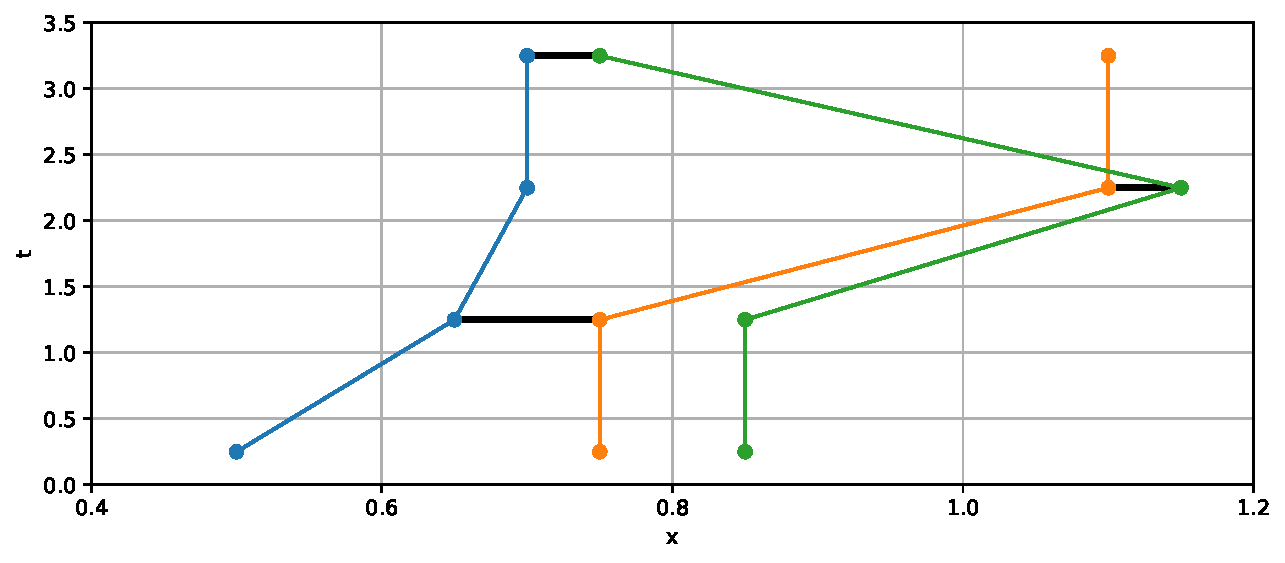
\includegraphics[width=12cm]{similar.pdf}
  \caption{Three trajectories with \(\locset = \R\) are shown. The
    grid represents the partitioning of \(\dataset\), where both time
    and space is partitioned into intervals of length 1. Datapoints
    which are in the same part of the grid are considered similar. For
    this co-trajectory there are three pairs for datapoints which are
    similar, denoted by the circles.}
  \label{fig:similar}
\end{figure}

While we do not restrict which partitioning is used for \(\locset\),
the choice of it, together with the choice of \(d\) for partitioning
\(\timeset\), is very important. If two datapoints are equivalent with
respect to the partitioning then swapping trajectories based on that
should does not give rise to too big jumps. What constitutes a too big
jump heavily depends on the setting and the type of datapoints. If we
for example only have datapoints hourly then fairly big jumps are
acceptable since an individual can move a lot in an hour, but if we
have datapoints for every minute much smaller jumps are reasonable. In
Figure \ref{fig:jumps} we can see an example of how the number of
datapoints influences which jumps are reasonable.

\begin{figure}
    \centering
    \begin{subfigure}[t]{0.45\textwidth}
      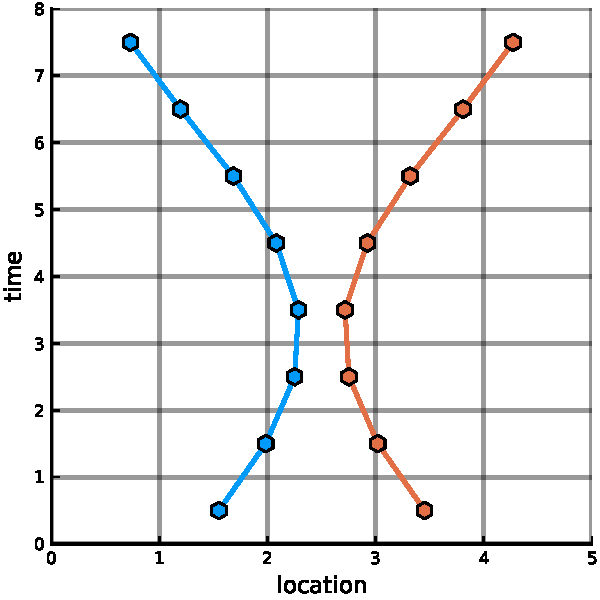
\includegraphics[width=6cm]{jumps-1a.pdf}
      \caption{}
      \label{fig:jumps-1a}
    \end{subfigure}
    \begin{subfigure}[t]{0.45\textwidth}
      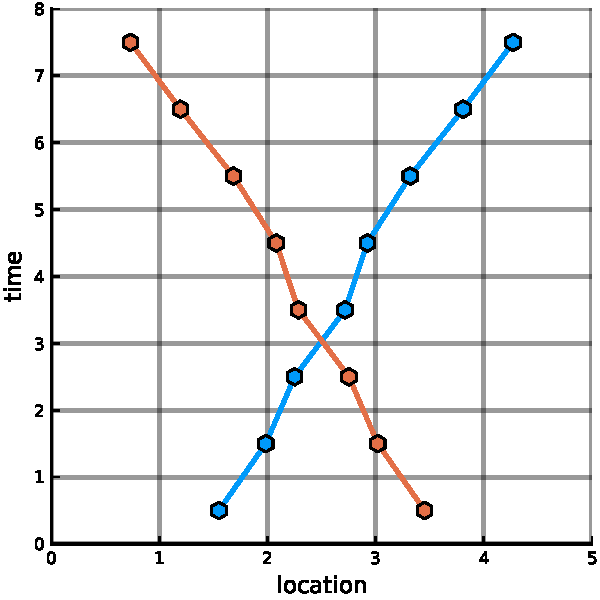
\includegraphics[width=6cm]{jumps-1b.pdf}
      \caption{}
      \label{fig:jumps-1b}
    \end{subfigure}

    \begin{subfigure}[t]{0.45\textwidth}
      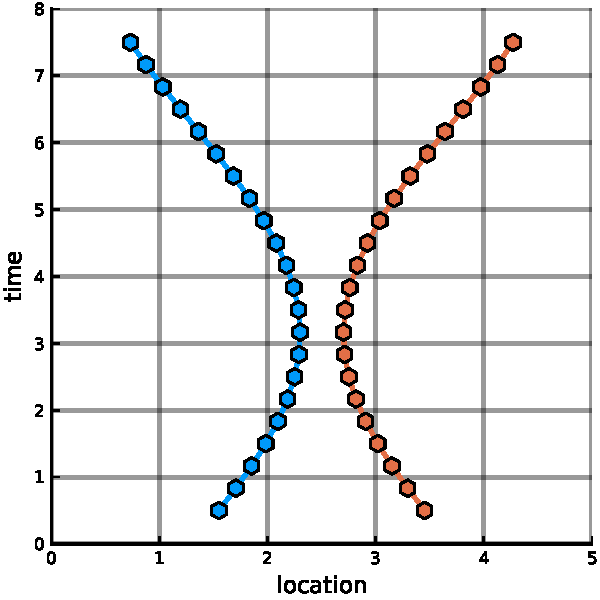
\includegraphics[width=\textwidth]{jumps-2a.pdf}
      \caption{}
      \label{fig:jumps-2a}
    \end{subfigure}
    \begin{subfigure}[t]{0.45\textwidth}
      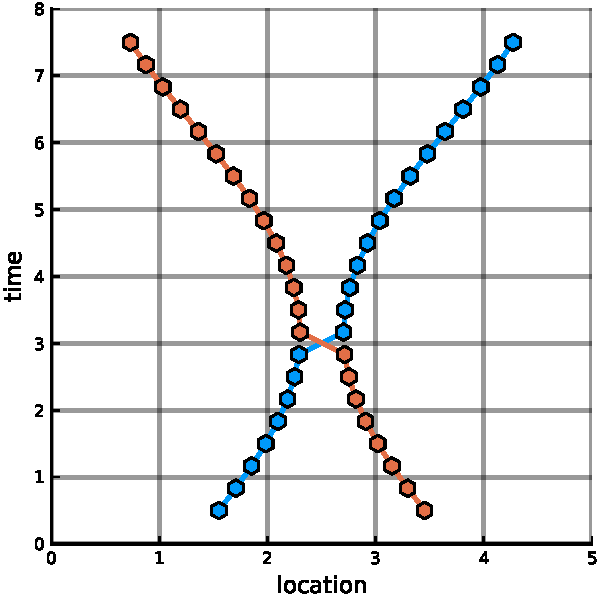
\includegraphics[width=\textwidth]{jumps-2b.pdf}
      \caption{}
      \label{fig:jumps-2b}
    \end{subfigure}
    \caption{The number of datapoints influences which jumps are
      reasonable. We see the same trajectories but with different
      number of datapoints. The same valid swap is performed in both
      cases at the time \(\swaptime = 3\). In (a) and (b) the swap
      looks reasonable and is not to obvious whereas in (c) and (d) it
      is very clear where the swap is performed and we have a big jump
      for the trajectories. This indicates that the partitioning for
      (c) and (d) should be made finer to avoid swaps with to big
      jumps.}
    \label{fig:jumps}
\end{figure}

\subsubsection{Swapping for co-trajectories}
We now go through the process of defining swapping for co-trajectories
where there are more than two trajectories involved. First we define
swapping for multiple trajectories and which swaps are valid for
co-trajectories. Then we discuss how to perform several swaps on a
co-trajectory and how the order the swaps are performed in affects the
outcome.

Swaps for co-trajectories is defined similar to swaps between pairs of
trajectories. Given a co-trajectory
\(\cotraj = \{\traj_{i}\}_{i = 1}^{N}\), a swap at time \(\swaptime\)
is given by a permutation \(\pi \in S_{N}\) and gives the
co-trajectory \(\overline{\cotraj}\) given by
\(\{\overline{\traj}_{i}\}_{i = 1}^{N}\), where
\begin{equation}
  \label{eq:swap-cotrajectory}
  \overline{\traj}_{i} = \{(\loc, \tim) \in \traj_{i}: \tim < \swaptime\} \cup \{(\loc, \tim) \in \traj_{\pi(i)}: \tim \geq \swaptime\},\ i = 1, 2, \dots, n.
\end{equation}
So \(\overline{\traj}_{i}\) has the datapoints from \(\traj_{i}\)
before time \(\swaptime\) and from \(\traj_{\pi(i)}\) starting from
time \(\swaptime\). A swap is uniquely defined by its time \(\swaptime\)
and permutation \(\pi\) and we denote a swap by
\(\swap = (\swaptime, \pi)\).

For a swap \(s = (\swaptime, \pi)\) of a co-trajectory to be valid we
require that all the trajectories in the support of \(\pi\), i.e. all
\(\traj_{i}\) such that \(\pi(i) \not= i\), have datapoints which
are similar and that the swap occurs right after the time for the
datapoints equivalence class.

\begin{definition}[\textbf{Co-trajectory Valid Swap}]
  A swap \(\swap = (\swaptime, \pi)\) on a co-trajectory
  \(\cotraj = \{\traj_{i}\}_{i = 1}^{N}\) is called a valid swap if
  \(\swaptime = \sup(\timint)\) and there exists an equivalence class
  \(\locint \times \timint\) such that for all \(i\) in the support of
  \(\pi\) there exists \(\data_{i} \in \traj_{i}\) with
  \(\data_{i} \in \locint \times \timint\) with .
\end{definition}

Next we discuss how to perform multiple swaps on a co-trajectory. Let
\(\cotraj_{0}\) be a co-trajectory and
\(\swap_{1}, \swap_{2}, \dots, \swap_{n}\) be swaps on it. One way to
perform all of these swaps is to do them one after another. Performing
\(\swap_{1}\) on \(\cotraj_{0}\) gives us a new co-trajectory
\(\cotraj_{1}\), on this new co-trajectory we can then perform
\(\swap_{2}\) giving us \(\cotraj_{2}\). In general we get \(n\) new
co-trajectories \(\cotraj_{i}\) for \(1 \leq i \leq n\), where
\(\cotraj_{i}\) is given by performing the swap \(\swap_{i}\) on
\(\cotraj_{i-1}\). However, for valid swaps chaining them in this way
gives rise to problems, even if
\(\swap_{1}, \swap_{2}, \dots, \swap_{n}\) are all valid swaps for
\(\cotraj_{0}\) we might have that \(s_{i}\) is not a valid swap for
\(\cotraj_{i - 1}\) on which it is performed. See Figure
\ref{fig:swap-order} for an example of when this is the case. When
chaining the swaps we therefore have to take this into account.

To understand how to chain the swaps we have to consider at what a
valid swap does. For a valid swap \(\swap = (\swaptime, \pi\) with
support \(I\) we have datapoints \(\data_{i} \in \traj_{i}\) for
\(i \in I\) which are all similar, i.e. in the same equivalence class.
The swap \(\swap\) permutes datapoints between these trajectories.
Datapoints from the trajectory with \(\data_{i}\), in this case
\(\traj_{i}\), which occur after time \(\swaptime\) goes to the
trajectory having \(\data_{\pi^{-1}(i)}\), in this case
\(\traj_{\pi^{-1}(i)}\). We want to preserve this behaviour.

If we perform a swap \(\swap' = (\swaptime', \pi')\) before \(\swap\)
then \(\data_{i}\) and \(\data_{\pi^{-1}(i)}\) might have moved, and
if so we need to update \(\swap\) to take this into account. If
\(\swaptime \leq \swaptime'\) then neither \(\data_{i}\) nor
\(\data_{\pi^{-1}(i)}\) will be moved by \(\swap'\) (since they both
occur before time \(\swaptime\)), \(\swap\) will still be a valid swap
and we don't have to update it. If \(\swaptime > \swaptime'\) then
both of them will be moved, \(\data_{i}\) will belong to the
trajectory \(\traj_{\pi'^{-1}(i)}\) and \(\data_{\pi^{-1}(i)}\) to the
trajectory \(\traj_{\pi'^{-1}(\pi^{-1}(i))}\). To preserve the above
statement we want \(\swap\) to move datapoints from the trajectory
containing \(\data_{i}\), which now is \(\traj_{\pi'^{-1}(i)}\), to
the trajectory containing \(\data_{\pi^{-1}(i)}\), now
\(\traj_{\pi'^{-1}(\pi^{-1}(i))}\). For this we need a permutation
\(\pi''\) satisfying
\begin{equation*}
  \pi''(\pi'^{-1}(\pi^{-1}(i))) = \pi'^{-1}(i).
\end{equation*}
For this to hold for all \(i\) we need
\begin{equation}
  \label{eq:swap-update}
  \pi'' \circ \pi'^{-1} \circ \pi^{-1} = \pi'^{-1}
  \iff \pi'' = \pi'^{-1} \circ \pi \circ \pi'.
\end{equation}
We therefore replace the permutation \(\pi\) for \(\swap\) with the
permutation \(\pi'' = \pi'^{-1} \circ \pi \circ \pi'\).

To summarize, if we are to perform the valid swaps
\(\swap_{1}, \dots, \swap_{n}\) on the co-trajectory \(\cotraj_{0}\)
we start by performing \(\swap_{1}\) on it, giving us \(\cotraj_{1}\),
then, for all swaps \(\swap_{2}, \dots, \swap_{n}\) which occur after
\(\swap_{1}\) in time we update the permutation of them to
\(\pi_{1}^{-1} \circ \pi_{i} \circ \pi_{1}\). This ensures that all
the swaps are valid swaps on \(\cotraj_{1}\). We then continue by
performing the updated \(\swap_{2}\) and updating the swaps
\(\swap_{3}, \dots, \swap_{n}\), we continue like this until all swaps
have been performed. This ensures that all the performed swaps are
valid on swaps on the co-trajectory that they are applied to. See
Figure \ref{fig:swap-order} for an example of this procedure.

\begin{figure}
    \centering
    \begin{subfigure}[t]{0.45\textwidth}
      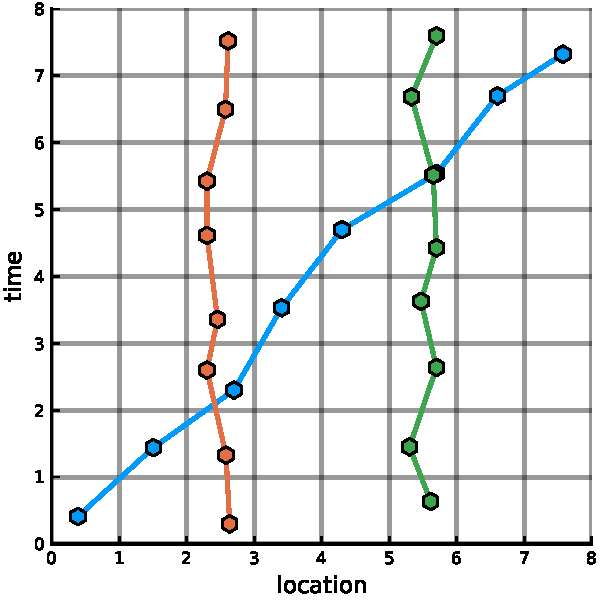
\includegraphics[width=6cm]{swaporder-a.pdf}
      \caption{Original co-trajectory}
      \label{fig:swap-order-a}
    \end{subfigure}
    \begin{subfigure}[t]{0.45\textwidth}
      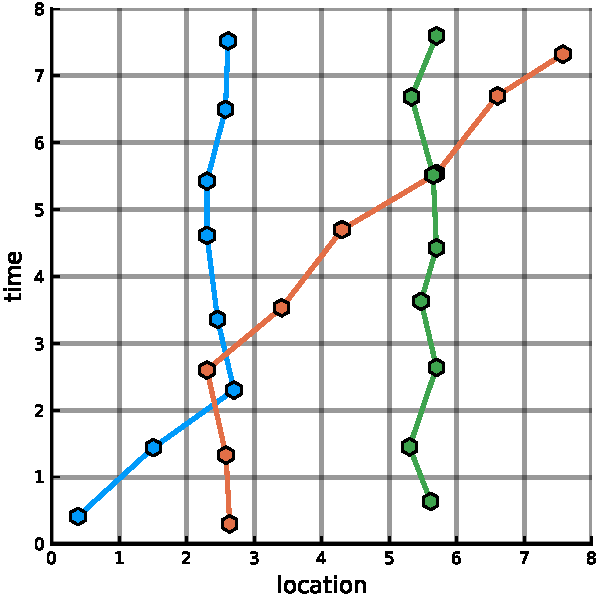
\includegraphics[width=6cm]{swaporder-b.pdf}
      \caption{Co-trajectory after first swap}
      \label{fig:swap-order-b}
    \end{subfigure}

    \begin{subfigure}[t]{0.45\textwidth}
      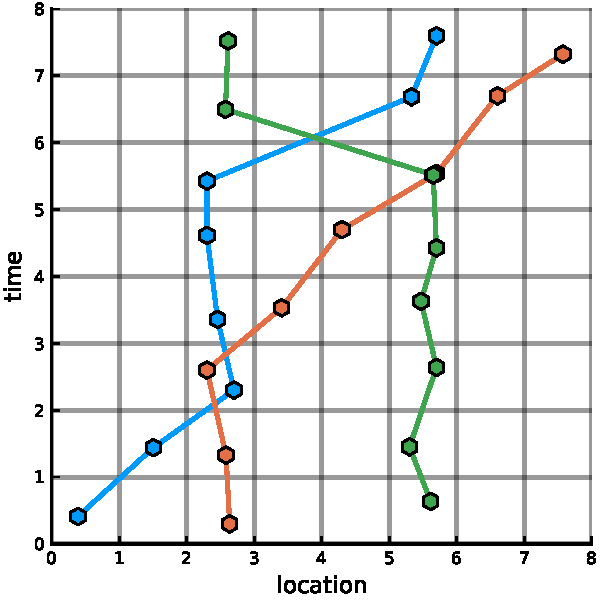
\includegraphics[width=\textwidth]{swaporder-c.pdf}
      \caption{Co-trajectory after second swap, without updating the
        swap}
      \label{fig:swap-order-c}
    \end{subfigure}
    \begin{subfigure}[t]{0.45\textwidth}
      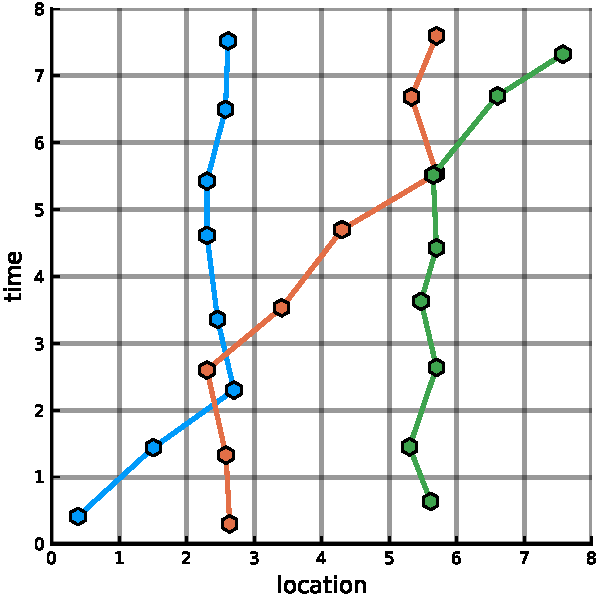
\includegraphics[width=\textwidth]{swaporder-d.pdf}
      \caption{Co-trajectory after second swap, updating the swap
        first}
      \label{fig:swap-order-d}
    \end{subfigure}
    \caption{The co-trajectory in (a) has two valid swaps,
      \(\swap_{1}\) which swaps \(\traj_{1}\) and \(\traj_{2}\) at
      time \(\swaptime = 3\) and \(\swap_{2}\) which swaps
      \(\traj_{1}\) and \(\traj_{3}\) at time \(\swaptime = 6\). In
      (b) \(\swap_{1}\) has been performed and for this co-trajectory
      \(\swap_{2}\) is no longer valid, instead \(\swap_{2}'\) which
      swaps \(\traj_{2}\) and \(\traj_{3}\) at time \(\swaptime = 6\)
      is valid. Performing \(\swap_{2}\) gives the result in (c)
      whereas performing \(\swap_{2}'\) the result in (d). If
      \(\pi_{1},\ \pi_{2}\) and \(\pi_{2}'\) are the permutations for
      \(\swap_{1},\ \swap_{2}\) and \(\swap_{2}'\) respectively we
      have that
      \(\pi_{2}' = \pi_{1}^{-1} \circ \pi_{2} \circ \pi_{1}\), as
      given by \ref{eq:swap-update}.}
    \label{fig:swap-order}
\end{figure}

We now discuss how the order swaps are performed in affect the
outcome. We show that the order of swaps occurring at different times
doesn't affect the outcome but that the order of swaps occurring at
the same time can affect the outcome.

\begin{lemma}
  \label{lemma:swap-order}
  Let \(\cotraj\) be a co-trajectory and consider two valid swaps,
  \(\swap = (\swaptime, \pi)\) and \(\swap' = (\swaptime', \pi'\), If
  \(\swaptime \not= \swaptime'\) then swapping first with \(\swap\)
  follower by \(\swap'\) gives the same result as swapping first with
  \(\swap'\) followed by \(\swap\).
\end{lemma}

\begin{proof}
  Without loss of generality assume that \(\swaptime < \swaptime'\).
  Let \(\cotraj^{\swap} = \{\traj^{\swap}_{i}\}_{i = 1}^{N}\) be the
  co-trajectory given by performing the swap \(\swap\) on \(\cotraj\)
  and \(\cotraj^{\swap'} = \{\traj^{\swap'}_{i}\}_{i = 1}^{N}\) the
  one given by performing \(\swap'\). Similarly let
  \(\cotraj^{\swap\swap'} = \{\traj^{\swap\swap'}_{i}\}_{i = 1}^{N}\)
  be the co-trajectory given by performing the \(\swap'\) on the
  co-trajectory \(\cotraj^{\swap}\), in this case we also first update
  \(\swap'\) according to Equation \ref{eq:swap-update}, and let
  \(\cotraj^{\swap'\swap} = \{\traj^{\swap'\swap}_{i}\}_{i = 1}^{N}\)
  be the co-trajectory given by performing \(\swap\) on
  \(\cotraj^{\swap'}\), in this case we don't need to update \(\swap\)
  since it occurs before \(\swap'\) in time. We have to show that
  \(\cotraj^{\swap\swap'} = \cotraj^{\swap'\swap}\), which we do by
  showing that \(\traj_{i}^{\swap\swap'} = \traj_{i}^{\swap'\swap}\)
  for all \(1 \leq i \leq N\).

  Let \(1 \leq i \leq N\), from Equation \ref{eq:swap-update} we get
  that the permutation for \(\swap'\), when performed after \(\swap\),
  is given by \(\pi^{-1} \circ \pi' \circ \pi\) which gives us that
  \(\traj^{\swap\swap'}_{i}\) is given by
  \begin{equation}
    \label{eq:order-1}
    \traj^{\swap\swap'}_{i} = \{(x, t) \in \traj^{\swap}_{i}: t < u'\}
    \cup \{(x, t) \in \traj^{\swap}_{\pi^{-1} \circ \pi' \circ \pi(i)}: t \geq u'\}.
  \end{equation}

  Here \(\traj^{\swap}_{i}\) is given by
  \begin{equation*}
    \traj^{\swap}_{i} = \{(x, t) \in \traj_{i}: t < u\}
    \cup \{(x, t) \in \traj_{\pi(i)}: t \geq u\},
  \end{equation*}
  and \(\traj^{\swap}_{\pi^{-1} \circ \pi' \circ \pi(i)}\) by
  \begin{equation*}
    \traj^{\swap}_{\pi^{-1} \circ \pi' \circ \pi(i)} = \{(x, t) \in \traj_{\pi^{-1} \circ \pi' \circ \pi(i)}: t < u\}
    \cup \{(x, t) \in \traj_{\pi(\pi^{-1} \circ \pi' \circ \pi(i))}: t \geq u\}.
  \end{equation*}
  Putting this into Equation \ref{eq:order-1} gives
  \begin{align}
    \begin{split}
      \label{eq:order-1-final}
      \traj^{\swap\swap'}_{i} &= \{(x, t) \in \traj^{\swap}_{i}: t < u'\}
      \cup \{(x, t) \in \traj^{\swap}_{\pi^{-1} \circ \pi' \circ \pi(i)}: t \geq u'\}\\
      &= \{(x, t) \in \traj_{i}: t < u\}
      \cup \{(x, t) \in \traj_{\pi(i)}: u \leq t < u'\}\\
      &\qquad \cup \{(x, t) \in \traj_{\pi(\pi^{-1} \circ \pi' \circ \pi(i))}: t \geq u'\}.
    \end{split}
  \end{align}

  For \(\traj^{\swap'\swap}_{i}\) we get
  \begin{equation}
    \label{eq:order-2}
    \traj^{\swap'\swap}_{i} = \{(x, t) \in \traj^{\swap'}_{i}: t < u\}
    \cup \{(x, t) \in \traj^{\swap'}_{\pi(i)}: t \geq u\}
  \end{equation}
  Here \(\traj^{\swap'}_{i}\) is given by
  \begin{equation*}
    \traj^{\swap'}_{i} = \{(x, t) \in \traj_{i}: t < u'\}
    \cup \{(x, t) \in \traj_{\pi'(i)}: t \geq u'\},
  \end{equation*}
  and \(\traj^{\swap'}_{\pi(i)}\) by
  \begin{equation*}
    \traj^{\swap'}_{\pi(i)} = \{(x, t) \in \traj_{\pi(i)}: t < u'\}
    \cup \{(x, t) \in \traj_{\pi'(\pi(i))}: t \geq u'\}.
  \end{equation*}
  Putting this into Equation \ref{eq:order-2} gives us
  \begin{align}
    \begin{split}
      \label{eq:order-2-final}
      \traj^{\swap'\swap}_{i} &= \{(x, t) \in \traj^{\swap'}_{i}: t < u\}
      \cup \{(x, t) \in \traj^{\swap'}_{\pi(i)}: t \geq u\}\\
      &= \{(x, t) \in \traj_{i}: t < u\}
      \cup \{(x, t) \in \traj_{\pi(i)}: u \leq t < u'\}\\
      &\qquad \cup \{(x, t) \in \traj_{\pi'(\pi(i))}: t \geq u'\}.
    \end{split}
  \end{align}

  Since \(\pi(\pi^{-1} \circ \pi' \circ \pi(i)) = \pi'(\pi(i))\) we
  get from Equation \ref{eq:order-1-final} and \ref{eq:order-2-final}
  that \(\traj^{\swap\swap'}_{i} = \traj^{\swap'\swap}_{i}\). Since we
  made no assumption on \(i\) this should hold for all
  \(1 \leq i \leq N\) and thus
  \(\cotraj^{\swap\swap'} = \cotraj^{\swap'\swap}\) and we conclude
  that the order the swaps are performed in doesn't matter.
\end{proof}

\begin{proposition}
  \label{prop:swap-order}
  Let \(\cotraj\) be a co-trajectory and consider \(n\) valid swaps,
  \(\swap_{i}\) \(1 \leq i \leq n\), where
  \(\swap_{i} = (\swaptime_{i}, \pi_{i})\). If
  \(\swaptime_{i} \not= \swaptime_{j}\) for all \(i \not= j\), then
  the order the swaps are performed in doesn't change the result.
\end{proposition}

\begin{proof}
  Given any ordering of the swaps we can apply Lemma
  \ref{lemma:swap-order} to change the order of two swaps that are
  next to each other in the order without changing the final outcome.
  For example the ordering
  \(s_{1}, s_{2}, \dots, s_{i}, s_{i + 1}, \dots, s_{n}\) gives the
  same results as the ordering
  \(s_{1}, s_{2}, \dots, s_{i + 1}, s_{i}, \dots, s_{n}\) according to
  Lemma \ref{lemma:swap-order}.

  In turns of permutations this means that adjacent transpositions of
  the swaps, i.e. changing the order of two swaps next to each other,
  does not affect the result. Notice that we are here talking about
  permutations on the order of the swaps, not about the permutations
  the swaps perform. Since the set of all permutations of the swaps,
  \(S_{n}\), is generated by the set of adjacent transpositions we can
  get to any permutations of the swaps by iteratively applying
  adjacent transpositions. As non of the adjacent transpositions
  affect the result we get that the result of the final permutation is
  the same as the original one. We conclude that for all orderings of
  the swaps the results are the same.
\end{proof}

The above proposition shows that the order of swaps that occur at
different times doesn't matter. For swaps occurring at the same time
the order does matter, an example of this is seen in Figure
\ref{fig:swap-order-counter-example}. In general we get the following
result.

\begin{proposition}
  \label{prop:swap-compose}
  Let \(\cotraj\) be a co-trajectory and consider two valid swaps,
  \(\swap = (\swaptime, \pi)\) and \(\swap' = (\swaptime', \pi')\). If
  \(\swaptime = \swaptime'\) then performing the swap \(\swap\)
  followed by \(\swap'\) gives the same result as performing a single
  swap, \(\swap \circ \swap' = (\swaptime, \pi \circ \pi'\).
\end{proposition}

\begin{proof}
  Let \(\cotraj^{\swap} = \{\traj^{\swap}_{i}\}_{i = 1}^{N}\) be the
  co-trajectory given by performing the swap \(\swap\) on \(\cotraj\)
  and
  \(\cotraj^{\swap\swap'} = \{\traj^{\swap\swap'}_{i}\}_{i = 1}^{N}\)
  be the co-trajectory given by performing swap the \(\swap'\) on the
  co-trajectory \(\cotraj^{\swap}\). Notice that we do not need to
  update the permutation for \(\swap'\) since it occurs at the same
  time as \(\swap\). Also let
  \(\cotraj^{(\swap \circ \swap')} = \{\traj^{(\swap \circ
    \swap')}_{i}\}_{i = 1}^{N}\) be the co-trajectory given by
  performing the swap \(\swap \circ \swap'\) on \(\cotraj\). We show
  that \(\traj^{\swap\swap'}_{i} = \traj^{(\swap \circ \swap')}_{i}\)
  for all \(1 \leq i \leq N\).

  For all \(1 \leq i \leq N\) we have that
  \begin{equation*}
    \traj^{\swap}_{i} = \{(x, t) \in \traj_{i}: t < u\}
    \cup \{(x, t) \in \traj_{\pi(i)}: t \geq u\}.
  \end{equation*}
  and for \(\traj^{\swap\swap'}_{i}\) this gives us
  \begin{align*}
    \traj^{\swap\swap'}_{i} & = \{(x, t) \in \traj^{\swap}_{i}: t < u\}
                              \cup \{(x, t) \in \traj^{\swap}_{\pi'(i)}: t \geq u\}\\
                            & = \{(x, t) \in \traj_{i}: t < u\}
                              \cup \{(x, t) \in \traj_{\pi'(\pi(i))}: t \geq u\}.
  \end{align*}
  For \(\traj^{(\swap \circ \swap')}_{i}\) we get
  \begin{equation*}
    \traj^{(\swap \circ \swap')}_{i} = \{(x, t) \in \traj_{i}: t < u\}
    \cup \{(x, t) \in \traj_{(\pi \circ \pi')(i)}: t \geq u\}.
  \end{equation*}
  Since \((\pi \circ \pi')(i) = \pi(\pi'(i))\) we get that
  \(\traj^{\swap\swap'} = \traj^{{(\swap \circ \swap')}}\). It follows
  that \(\cotraj^{\swap\swap'} = \cotraj^{(\swap \circ \swap')}\).
\end{proof}

A consequence of this is that the order of the swaps doesn't matter as
long as the permutations for them commute with each other. One
particular case of this is when the supports for all the permutations
are disjoint, since then the permutations commute. In Figure
\ref{fig:swap-order-counter-example} the permutations for the swaps
does not commute and the order they are applied in does therefore
affect the result.

\begin{figure}
    \centering
    \begin{subfigure}[t]{0.45\textwidth}
      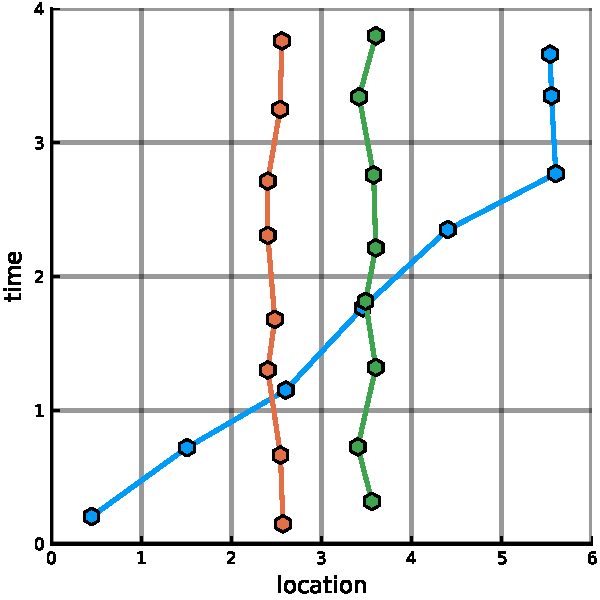
\includegraphics[width=6cm]{swaporder_counterexample-a.pdf}
      \caption{Original co-trajectory}
      \label{fig:swap-order-counter-example-a}
    \end{subfigure}

    \begin{subfigure}[t]{0.45\textwidth}
      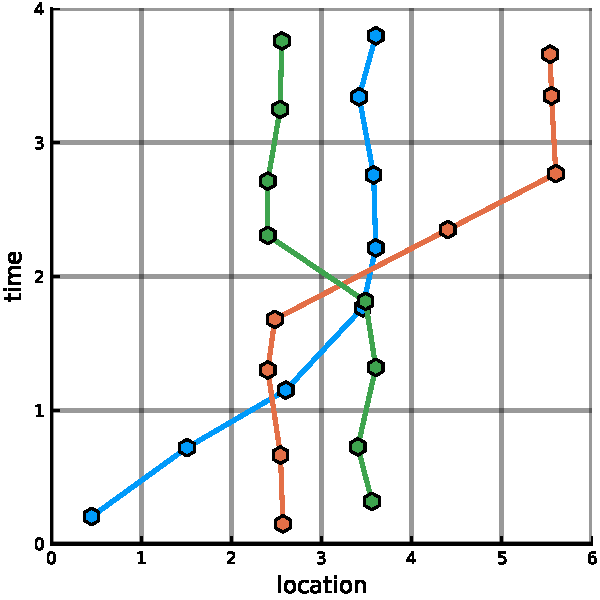
\includegraphics[width=6cm]{swaporder_counterexample-b.pdf}
      \caption{Swapping first with \(\swap\) and then with \(\swap'\)}
      \label{fig:swap-order-counter-example-b}
    \end{subfigure}
    \begin{subfigure}[t]{0.45\textwidth}
      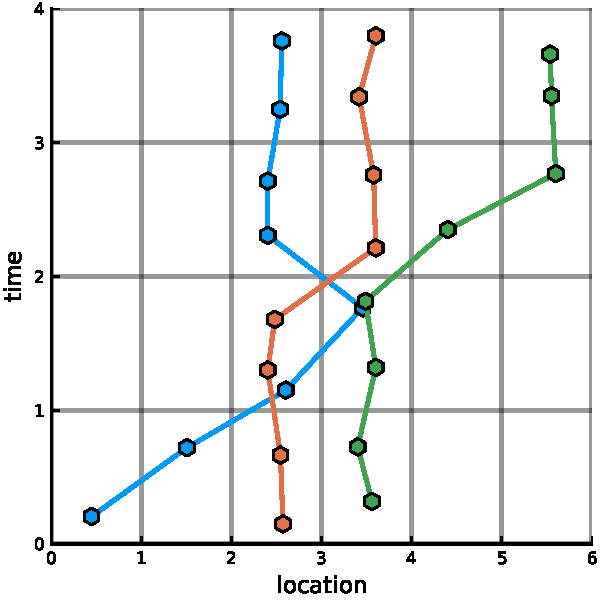
\includegraphics[width=\textwidth]{swaporder_counterexample-c.pdf}
      \caption{Swapping first with \(\swap'\) and then with \(\swap\)}
      \label{fig:swap-order-counter-example-c}
    \end{subfigure}
    \caption{The co-trajectory in (a) has two valid swaps, \(\swap\)
      which swaps \(\traj_{1}\) and \(\traj_{2}\) at time
      \(\swaptime = 2\) and \(\swap'\) which swaps \(\traj_{1}\) and
      \(\traj_{3}\) at the same time \(\swaptime = 2\). In (b) we see
      the result of first performing \(\swap\) and then \(\swap'\)
      whereas in (c) we see the result of performing them in the
      opposite direction.}
    \label{fig:swap-order-counter-example}
\end{figure}

How the order of swaps affect the outcome will have implications when
choosing which swaps to perform when using SwapMob, for details of
this see the Section \ref{sec:swapmob-algorithm} where the algorithm
for SwapMob is discussed.

\subsubsection{Comparison to mix-zones}
\label{sec:compare-mix-zones}
Of the methods mentioned in the beginning of Section \ref{sec:swapmob}
for protecting privacy when working with trajectories and
co-trajectories , the one that is most similar to SwapMob is mix-zones
\cite{beresford_location_2003, beresford_mix_2004}.

In the context of mix-zones every individual is associated with a
pseudonym, the mix-zones are certain areas for which the individual
change pseudonym when they enter. With our definitions of trajectories
and co-trajectories this corresponds to the individual being
associated with two different trajectories, one before entering the
zone and one after. This makes it harder to track the long term
movement of individuals since the data gets spread out between several
trajectories whenever they enter the mix-zones and it is hard to know
which trajectories belong to the same individual. For this to work
properly no data should be collected while the individual is inside
the mix-zone, otherwise it is easy to find which trajectories belong
together by looking at there first and final datapoint. In addition
there should be several individuals in the mix-zone at the same time
and it should be hard to correlate where and when you go into the
mix-zone with where and when you go out.

SwapMob and mix-zones are similar in that they both split the
datapoints of an individual among several trajectories to make it
harder to link them all together. For mix-zones this is done when the
individual enters a mix-zone and for SwapMob when two individuals come
close enough to perform a swap. This makes SwapMob more dynamic than
mix-zones, since it allows swapping anywhere whereas mix-zones are
more static.

For mix-zones no data should be collected while the individual is
inside the mix-zone, this improves the privacy since less data is
collected but also limits the usability of the data since no analysis
about what happens inside the mix-zone can be done.

For the individual the privacy gained from mix-zones could be more
clear. They could know how often they enter a mix-zone, and thus how
many times there trajectory is split up. Whereas for SwapMob it can be
hard for the individual to know how many swaps they participate it. To
know if you enter a mix-zone only depends on your own trajectory
whereas to know if you participate in a swap you have know both you
own trajectory and the trajectories of others. However for mix-zones
you might not know how many other people are in the mix-zone at the
same time, and thus how many other people you are mixed with.

To summarize, mix-zones and SwapMob are similar but with some key
differences. Mix-zones prohibits data collection in some areas whereas
SwapMob does not by itself prohibit data collection anywhere.
Mix-zones work with static areas for mixing trajectories whereas
SwapMob dynamically finds appropriate places for swapping
trajectories.

\subsection{Algorithm}
\label{sec:swapmob-algorithm}
In this section we give the algorithm for SwapMob, the main focus is
on the mathematical properties but some implementation details will
also be discussed. The algorithm is divided into two parts, the first
is about determining which swaps to perform and the second about how
to perform these swaps. Of these two parts the former is the more
interesting one and the one that will play a role in Section
\ref{sec:swapmob-analysis} when analysing the algorithm. We do however
start by giving the algorithm for performing the swaps, since some of
the remarks there have implications for which swaps we choose to
include when determining the swaps to use.

\subsubsection{Performing swaps}
The algorithm for performing swaps will take as input a co-trajectory
and a list of swaps to perform and return a new co-trajectory with all
the swaps performed.

We begin by giving an algorithm for performing a single swap on a
co-trajectory. The final algorithm will then be given by iterating
this for each swap to perform. To perform a swap we simply take the
original co-trajectory and for each trajectory in the support of the
swap we replace it with the resulting trajectory according to Equation
\ref{eq:swap-cotrajectory}.

\begin{algorithm}
  \caption{Algorithm for performing a single swap on a co-trajectory}
  \label{alg:swap-single}
  \begin{algorithmic}
    \Procedure{swapSingle}{$\cotraj, \swap = (\swaptime,\ \pi)$}
    \Comment{The co-trajectory resulting from performing the swap
      \(\swap\) on the co-trajectory \(\cotraj\)}
    \State \(\cotraj' \gets \cotraj\)
    \State \(I \gets support(\pi)\)
    \For{\(i \in I\)}
    \State \(part_{1} \gets \{(\loc, \tim): (\loc, \tim) \in
    \cotraj[i], \tim < \swaptime\}\)
    \State \(part_{2} \gets \{(\loc, \tim): (\loc, \tim) \in
    \cotraj[\pi(i)], \tim \geq \swaptime\}\)
    \State \(\cotraj'[i] \gets part_{1} \cup part_{2}\)
    \EndFor
    \State \textbf{return} \(\cotraj'\)
    \EndProcedure
  \end{algorithmic}
\end{algorithm}

When iterating this algorithm for all the swaps in the list we have to
take care about which order we perform the swaps in. According to
Proposition \ref{prop:swap-order} the result does not depend on the
ordering of swaps with different timestamps, the computational cost of
computing the result does however depend on the order, when performing
a swap we have to update all remaining swaps with a timestamp
occurring later than the current swap according to Equation
\ref{eq:swap-update}. By ordering the swaps so that the timestamps are
decreasing we avoid having to update any swaps, because when
performing a swap all remaining swaps have timestamps which are
occurring at the same time or before the one for the current swap, and
thus doesn't have to be updated.

Ordering by timestamp does however not solve the problem of how to
order swaps with the same timestamp. One option is to use a random
order, however, as discussed above and exemplified in Figure
\ref{fig:swap-order-counter-example}, the order does affect the
result. This would therefore introduce randomness in the swapping
procedure, which we would prefer to avoid. Another option is to use a
pre-specified order for them, but there is no natural choice to use
for the ordering. To handle this we begin by noticing that if the
permutations for all the swaps occurring at a specific timestamp all
commute, then the order they are performed in does not affect the
outcome as per Proposition \ref{prop:swap-compose}. In this case we
can choose a random order to perform them in without it affecting the
result. In particular, if the supports of the swaps occurring at the
same time are all disjoint then they commute. One solution is
therefore to require that the list of swaps, returned by the algorithm
that determines the swaps to perform, satisfies that every trajectory
participates in at most one swap for each timestamp, this ensures that
swaps occurring at the same time have disjoint support and thus
commute. By requiring this we are ensured that the order the swaps are
performed in does not matter.

The final algorithm begins by sorting the list of swaps so that the
timestamps are decreasing. It then takes the swaps one by one and
perform them on the co-trajectory using Algorithm
\ref{alg:swap-single}. This is seen in Algorithm \ref{alg:swap}.

\begin{algorithm}
  \caption{Algorithm for performing several swaps on a co-trajectory}
  \label{alg:swap}
  \begin{algorithmic}
    \Procedure{swap}{$\cotraj, swapList$}
    \Comment{The co-trajectory resulting from performing all the swaps
      in \(swapList\) on the co-trajectory \(\cotraj\)}
    \State \textbf{Sort} \(swapList\) \textbf{By decreasing timestamps}
    \For{\(\swap \in swapList\)}
    \State \(\cotraj \gets swapSingle(\cotraj, \swap)\)
    \EndFor
    \State \textbf{return} \(\cotraj\)
    \EndProcedure
  \end{algorithmic}
\end{algorithm}

\subsubsection{Determining swaps}
\label{sec:determining-swaps}

The algorithm for determining which swaps to perform takes as an
argument a co-trajectory and returns a list of swaps to be performed.
It is the composition of one deterministic and one randomized
algorithm. The first algorithm returns a list of groups of
trajectories according to their datapoints equivalence classes and
the second algorithm then chooses a random permutation to use for each
group.

The deterministic algorithm takes as input a co-trajectory,
\(\cotraj\), it groups the trajectories according to their datapoints
equivalent classes and returns these groups together with the supremum
time for the respective equivalence class. More precisely it returns a
list of elements on the form \((\swaptime, I)\), where \(I\) is a
(multi-)set of trajectories satisfying that there is an equivalence
class \(\locint \times \timint\) such that for all \(\traj_{i} \in I\)
there exists \(\data \in \traj_{i}\) with
\(\data \in \timint \times \locint\) and further
\(\swaptime = \sup(\timint)\). This ensures that any swap that
permutes the trajectories in \(I\) which occur at time \(\swaptime\)
is a valid swap.

From Algorithm \ref{alg:swap} we have the requirement that no
trajectory should participate in several swaps at the same time. This
means that for two returned elements \((\swaptime, I)\) and
\((\swaptime', I')\) we should have
\(\swaptime = \swaptime' \implies I \cap I' = \emptyset\). One simple
way to satisfy this is to only consider the last datapoint in every
time interval of a trajectory when finding valid swaps. This can be
accomplished by removing all the other datapoints from the
trajectories before finding the groups. Notice that since the
definition of a trajectory only allow for a finite number of
datapoints in every finite time interval we can be certain that there
is a well defined last datapoint in every interval.

The algorithm is given in Algorithm \ref{alg:group-trajectories}. It
begins by for every trajectory only keeping the last datapoint in
every time interval. It then collects a set of all remaining
datapoints in the co-trajectory, together with the id of the
trajectory they belong to. This set is then grouped according to the
equivalence class of the datapoints, giving a set where each element
is given by an equivalence class together with a set of ids
corresponding to datapoints that occurred in that equivalence class.
We discard any equivalence classes having only one id belonging to it,
since no swapping can be performed with just one trajectory. We then
return the groups of ids together with the time to swap them, i.e.
supremum time of their equivalence class.

\begin{algorithm}
  \caption{Deterministic part of algorithm for determining swaps}
  \label{alg:group-trajectories}
  \begin{algorithmic}
    \Procedure{GroupTrajectories}{$\cotraj$} \Comment{Groups of
      trajectories grouped according to equivalence classes of their
      datapoints}

    \State
    \(\cotraj' \gets \{\textrm{filter}(\traj_{i}): \traj_{i} \in
    \cotraj\}\)

    \State
    \(datapoints \gets \{(i,\ \data): \forall \data \in \traj_{i},
    \forall \traj_{i} \in \cotraj'\}\)

    \State
    \(groups_{1} \gets \{(\locint \times \timint, \{i: (i, \data) \in
    datapoints, \data \in \locint \times \timint\}): \forall \locint
    \times \timint\}\)

    \State
    \(groups_{2} \gets \{(\locint \times \timint, I) \in groups_{1}:
    |I| > 1\}\)

    \State \textbf{return}
    \(\{(\sup(\timint),\ I): (\timint \times \locint,\ I) \in
    groups_{2}\}\)

    \EndProcedure
  \end{algorithmic}
  \caption{Algorithm for computing groups of trajectories which have
    datapoints in the same equivalence class.}
\end{algorithm}

The second, randomized, algorithm associates each element in the list
returned by the first algorithm with a permutation, which, together
with the time, yields a swap. For the element \((\swaptime,\ I)\) the
permutation is chosen uniformly at random from all permutations
\(\pi \in S_{|\cotraj|}\) whose support is a subset of \(I\), this
ensures that the resulting swap, \(\swap = (\swaptime, \pi)\), is a
valid swap.

Composing Algorithm \ref{alg:group-trajectories} with this randomized
algorithm gives us an algorithm which takes a co-trajectory and
returns a list of valid swaps. This list of swaps can then be used as
an argument for Algorithm \ref{alg:swap} to perform the swapping.

\subsection{Analysis}
\label{sec:swapmob-analysis}
Having given the precise algorithm that SwapMob uses we continue with
analysing its properties. We analyse both what type of privacy the
swapping gives, what an adversary can learn from analysing the swapped
data, and what data is preserved under the swapping and how it can be
used in analysis.

Applying SwapMob to a co-trajectory, \(\cotraj\), gives as result a
new co-trajectory, \(\cotraj'\). The naive way to analyse \(\cotraj'\)
would be to see it as any other co-trajectory and use the same tools
for analysis. However, this would give us results for \(\cotraj'\) and
not \(\cotraj\), which is the co-trajectory we are interested in. We
need a way to take into account that SwapMob has been used to produce
\(\cotraj'\) and use this to get information about \(\cotraj\). The
main tool for this will be a representation of the swapped data as a
directed graph which encodes the effect of SwapMob.

\paragraph{SwapMob as a graph}
A trajectory can be represented as a directed acyclic graph (DAG) by
seeing the datapoints as vertices and putting edges between successive
datapoints, in fact this is how we have been visualizing trajectories
in most figures so far. Similarly a co-trajectory can be represented
by a DAG that is the union of DAG:s of trajectories. Swapping
trajectories corresponds to swapping the head of the edges. In Figure
\ref{fig:graph-swap-a} we see a co-trajectory and we can note that the
representation correspond to a DAG, in \ref{fig:graph-swap-b} a swap
has been performed and we can see that this correspond to changing the
heads of three edges. Instead of swapping with some specified
permutation we can encode the swap by creating a new vertex, a
swapping vertex, redirecting the heads to this vertex and creating new
edges from this vertex to the previous positions of the heads, the
result of this is seen in Figure \ref{fig:graph-swap-c}. Notice that
the resulting graph is also a DAG.

\begin{figure}
    \centering
    \begin{subfigure}[t]{0.3\textwidth}
      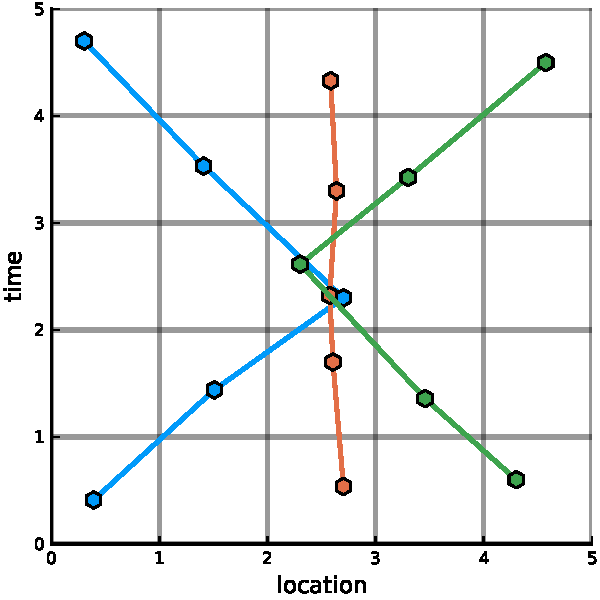
\includegraphics[width=\textwidth]{graph_swap-a.pdf}
      \caption{Original co-trajectory}
      \label{fig:graph-swap-a}
    \end{subfigure}
    \begin{subfigure}[t]{0.3\textwidth}
      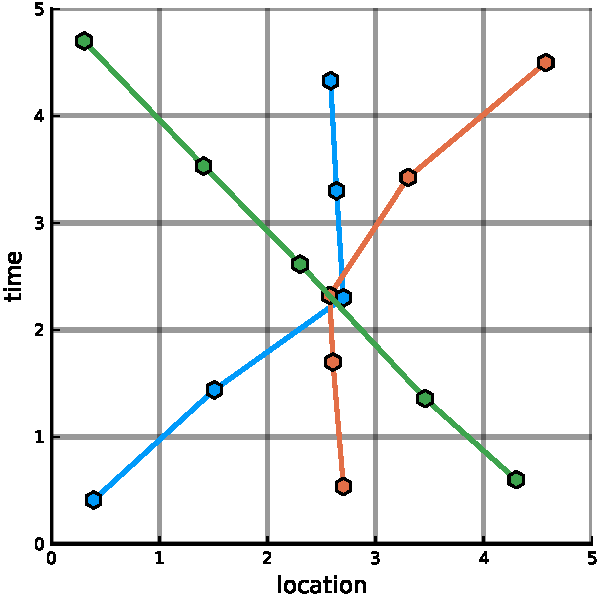
\includegraphics[width=\textwidth]{graph_swap-b.pdf}
      \caption{Co-trajectory after swapping}
      \label{fig:graph-swap-b}
    \end{subfigure}
    \begin{subfigure}[t]{0.3\textwidth}
      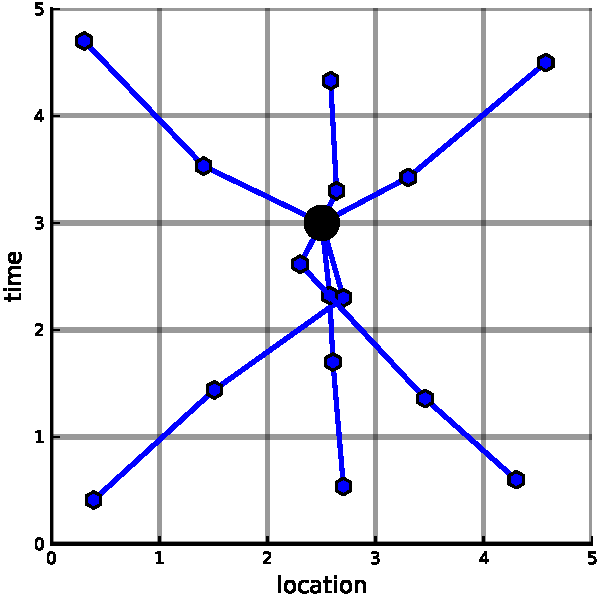
\includegraphics[width=\textwidth]{graph_swap-c.pdf}
      \caption{Co-trajectory with the swap as a vertex}
      \label{fig:graph-swap-c}
    \end{subfigure}
    \caption{The co-trajectory in (a) has a valid swap at time
      \(\swaptime = 3\). In (b) the co-trajectory resulting from
      performing the swap with the permutation \(\pi\) given by
      \(\pi(1) = 2\), \(\pi(2) = 3\), \(\pi(3) = 1\) is shown. Finally
      (c) shows the result of adding a new vertex to represent the
      swap. Notice that we in (c) no longer use different colors for
      the different trajectories, this is to highlight that this
      representation only keeps track of the topology of the
      co-trajectory and not the original trajectories.}
    \label{fig:graph-swap}
\end{figure}

If we have a number of swaps on a co-trajectory we can create swapping
vertices for all of them in this way. This is well defined as long as
no trajectory participate in several swaps at the same timestamp. In
fact we don't even need the permutations from the swaps, only the time
it should occur and which trajectories should participate. This means
that we can use the output from Algorithm \ref{alg:group-trajectories}
to generate the graph, Figure \ref{fig:graph-swap-full} shows an
example of this.

\begin{figure}
    \centering
    \begin{subfigure}[t]{0.45\textwidth}
      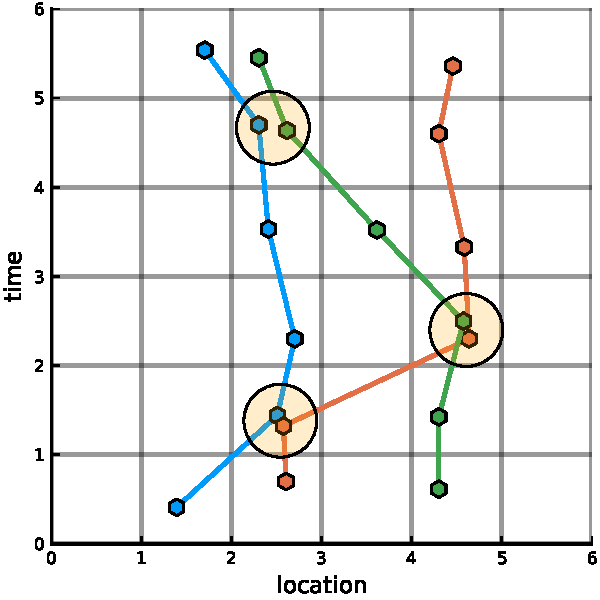
\includegraphics[width=\textwidth]{graph_swap_full-a.pdf}
      \caption{Original co-trajectory}
      \label{fig:graph-swap-full-a}
    \end{subfigure}
    \begin{subfigure}[t]{0.45\textwidth}
      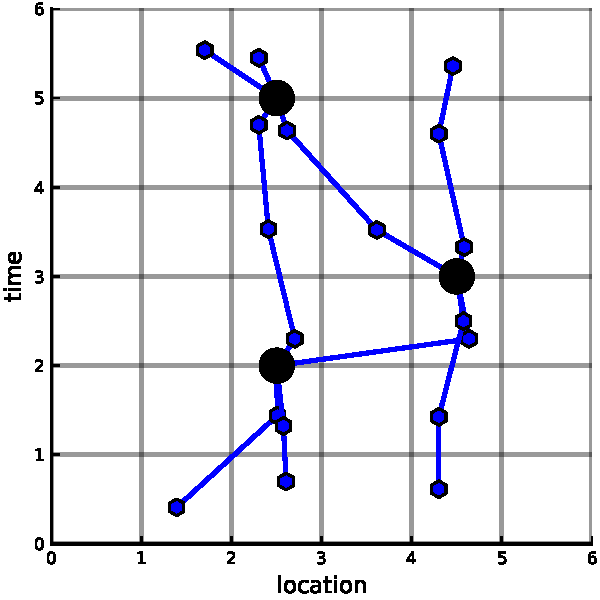
\includegraphics[width=\textwidth]{graph_swap_full-b.pdf}
      \caption{DAG representation of swapping}
      \label{fig:graph-swap-full-b}
    \end{subfigure}
    \caption{The co-trajectory in (a) has three valid swaps. In (b)
      all of these are represented by adding vertices to the graph,
      similarly to Figure \ref{fig:graph-swap-c} the trajectories are
      no longer shown with different colors.}
    \label{fig:graph-swap-full}
\end{figure}

For a co-trajectory \(\cotraj\) we denote by \(\graph(\cotraj)\) the
graph representation of the co-trajectory, such as the one seen in
Figure \ref{fig:graph-swap-full-a}, and by \(\swapgraph(\cotraj\)) the
graph representation with vertices for the swaps added. When the
\(\cotraj\)) is clear from the context we sometimes drop it and use
only \(\graph\) and \(\swapgraph\).

One of the important properties \(\swapgraph\) is that it is invariant
under SwapMob, i.e. for a co-trajectory \(\cotraj\) and a
co-trajectory \(\cotraj'\) given by applying SwapMob to \(\cotraj\)
the graphs \(\swapgraph(\cotraj\)) and \(\swapgraph(\cotraj'\)) are
identical. To see this consider the graph representations of the two
co-trajectories, \(\graph(\cotraj)\) and \(\graph(\cotraj')\), they
are identical except that the heads for the edges where swaps occur
are moved (as in Figure \ref{fig:graph-swap-a} and
\ref{fig:graph-swap-b}). The graphs \(\swapgraph(\cotraj)\) and
\(\swapgraph(\cotraj')\) will thus be the same since the head of the
edges that are moved in \(\graph(\cotraj')\) compared to
\(\graph(\cotraj)\) will be moved to the same new swap vertices
anyway, meaning that the difference between \(\graph(\cotraj)\) and
\(\graph(\cotraj')\) will not affect the \(\swapgraph\).

Every trajectory in \(\cotraj\) will correspond to paths in
\(\swapgraph(\cotraj)\). The opposite is not true, every path in
\(\swapgraph(\cotraj)\) will not correspond to a trajectory in
\(\cotraj\), however it will correspond to a possible trajectory after
swapping. A path makes a ``choice'' at every swapping node as to which
edge to follow, by choosing a permutation for each swapping node that
agrees with this choice we get as a result of the swapping a
co-trajectory with this trajectory in it. An example of this is seen
in Figure \ref{fig:graph-swap-full-c}. By considering the set of all
paths in \(\swapgraph(\cotraj)\) we can get the set of all possible
trajectories which we can get by swapping, in particular all
trajectories in the original co-trajectory are in this set.

\begin{figure}
  \centering
  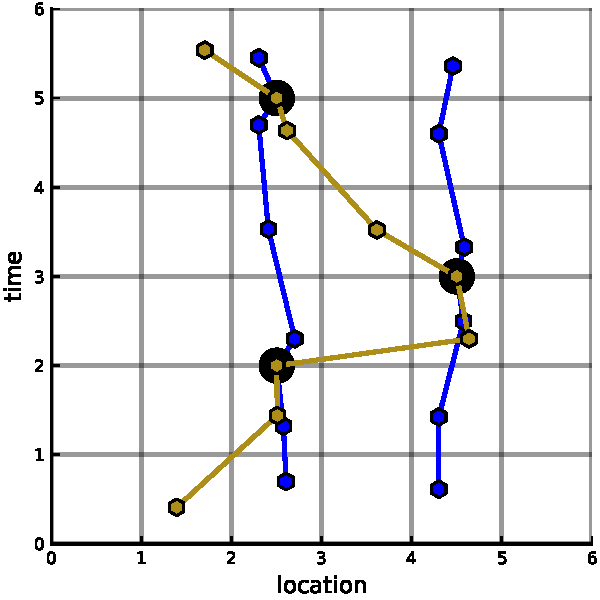
\includegraphics[width=6cm]{graph_swap_full-c.pdf}
  \caption{One possible path in Figure \ref{fig:graph-swap-full-b} is
    highlighted in yellow. This particular path does not appear in the
    original co-trajectory from \ref{fig:graph-swap-full-a} but could
    exist as a result of applying SwapMob if the right permutations
    are chosen.}
  \label{fig:graph-swap-full-c}
\end{figure}

\subsubsection{Privacy}
Let \(\cotraj\) be a co-trajectory and \(\cotraj'\) the resulting
co-trajectory from applying SwapMob to it. In this section we are
concerned about what data can be extracted about individuals in
\(\cotraj\) by an adversary having access to \(\cotraj'\). The main
observation is that since \(\swapgraph\) is invariant under SwapMob
the adversary will by having access to only \(\cotraj'\) still be able
to compute \(\swapgraph(\cotraj)\) since it is the same as
\(\swapgraph(\cotraj')\). By analysing \(\swapgraph(\cotraj)\) it can
gain information about trajectories in \(\cotraj\).

We consider the case of the adversary having access to different kinds
of partial data about an individual and what more it can learn about
the individual using the data from \(\cotraj'\).

As discussed in Section \ref{sec:priv-co-traj} one way to model the
partial data the adversary has is by considering a predicate,
\(\pred\), on trajectories, which returns true for trajectories
satisfying the partial data and false for those that don't. If the
adversary had access to the original co-trajectory, \(\cotraj\), it
would be enough to use the predicate on all trajectories in it to get
the possible trajectories for the individual. However the adversary
only have access to \(\cotraj'\) and must use this data together with
the knowledge that it was generated by applying SwapMob to the
original data. The original trajectory for the individual will most
likely not be in \(\cotraj'\), this is the case as long as it
participated in at least one swap. However, the original trajectory
will appear as a path in \(\swapgraph(\cotraj)\), which the adversary
has access to. The adversary can thus enumerate all paths in the graph
and use the predicate on all of them.

In more formal terms, let \(\paths\) denote the set of trajectories
corresponding to the set of all paths in \(\swapgraph(\cotraj)\), this
corresponds to the set of all trajectories we can get by swapping, and
as discussed above this set does in particular contain all
trajectories of the original co-trajectory \(\cotraj\). The adversary
can apply the predicate \(\pred\) to the trajectories in \(\paths\) to
get the set of all trajectories that could belong to the individual.
We denote by \(\pred(\paths)\) the set of all trajectories in
\(\paths\) that satisfy the predicate \(\pred\). The adversary knows
that the original trajectory is in this set.

How much privacy SwapMob gives with respect to a specific predicate
can then be measured by comparing the two sets \(\pred(\cotraj)\), the
information gained if SwapMob is not used, and \(\pred(\paths)\), the
information gained if SwapMob is used. The simplest comparison is to
look at the number of trajectories in the two sets, this corresponds
to the \(k\)-anonymity introduced in Section \ref{sec:priv-co-traj}.
The larger that \(|\pred(\paths))|\) is compared to
\(|\pred(\cotraj)|\) the more privacy is gained through SwapMob. How
much it increases will depend on the number of swaps for the
co-trajectory as well as the predicate.

Only comparing the number of trajectories does however not take into
account one of the important differences between \(\cotraj\) and
\(\paths\). In \(\cotraj\) all the trajectories correspond to
different individuals and do in general not share datapoints. For
\(\paths\) this is not the case, here a lot of the trajectories will
share datapoints since they are constructed by concatenating parts of
the trajectories from \(\cotraj\). For example we can see that the
outlined trajectory in \ref{fig:graph-swap-full-c} shares datapoints
will all the original trajectories seen in Figure
\ref{fig:graph-swap-full-a}. Therefore even if the \(k\)-anonymity is
increased a lot when comparing \(\pred(\cotraj)\) and
\(\pred(\paths)\) the diversity between the two sets might not, this
corresponds to the \(l\)-diversity not increasing a lot. The diversity
of \(\pred(\paths)\) could be measured in different ways, one simple
way would be to look at the intersection of all the trajectories to
find datapoints that occur in all of them and thus for sure belong to
the individual. As mentioned in Section \ref{sec:measuring-privacy} we
do not attempt to given a formal definition for measuring diversity
and keep the discussions about it on an informal level.

Another aspect that should be taken into account is the probability
for each permutation at a swap. For example consider the adversary
having access to the graph in Figure \ref{fig:u-turn-a}. The adversary
does not know the original co-trajectory, but knows that it was either
the one in Figure \ref{fig:u-turn-b} or \ref{fig:u-turn-c}. In Figure
\ref{fig:u-turn-b} the two trajectories both go in straight paths in
opposite directions whereas in Figure \ref{fig:u-turn-c} they go in
opposite directions and when they meet they both perform a complete
U-turn. In this scenario an adversary might consider the first case
more likely, that both trajectories continue on the way they were on.
It might seem less likely that both trajectories do a U-turn at the
same time. Another example would be when number of datapoints and the
partitioning doesn't align well, as in Figure \ref{fig:jumps}, in
which case the adversary can also see that one permutation is more
likely than the other. In the general case the adversary can use any
outside information to obtain a probability distribution for the
permutations at a swap node, with no information you get the uniform
distribution but with more information you could find permutations
which are more likely than others. In the extreme case the adversary
is able to determine with a very high probability which permutation
was performed at a swap node. This would mean that for a predicate
\(\pred\) all paths in \(\pred(\paths\) are not equally likely, some
might be much more likely and other much less. In the analysis below
this is not taken into account, indirectly we are assuming that the
adversary cannot infer anything about which permutations are more
likely.

\begin{figure}
    \centering
    \begin{subfigure}[t]{0.3\textwidth}
      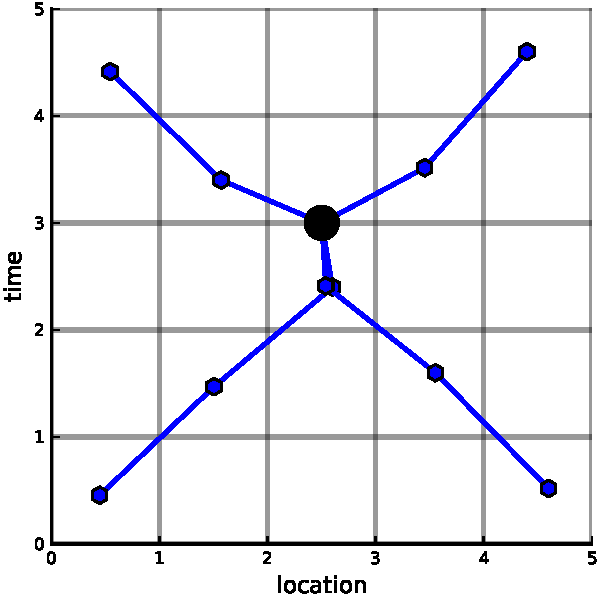
\includegraphics[width=\textwidth]{uturn-a.pdf}
      \caption{}
      \label{fig:u-turn-a}
    \end{subfigure}
    \begin{subfigure}[t]{0.3\textwidth}
      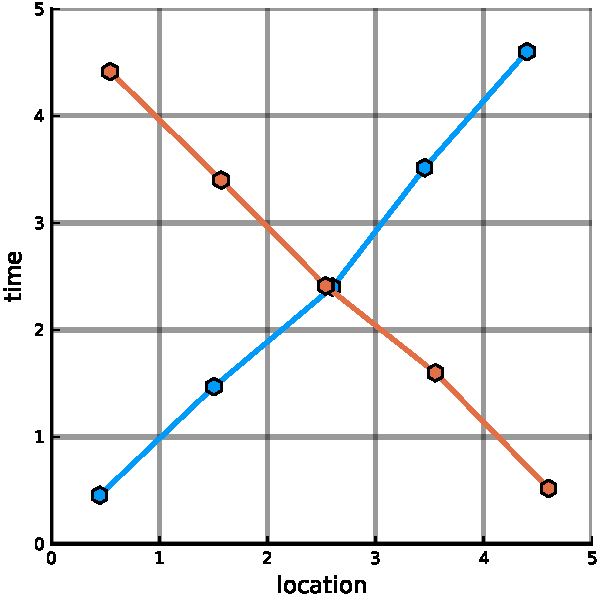
\includegraphics[width=\textwidth]{uturn-b.pdf}
      \caption{}
      \label{fig:u-turn-b}
    \end{subfigure}
    \begin{subfigure}[t]{0.3\textwidth}
      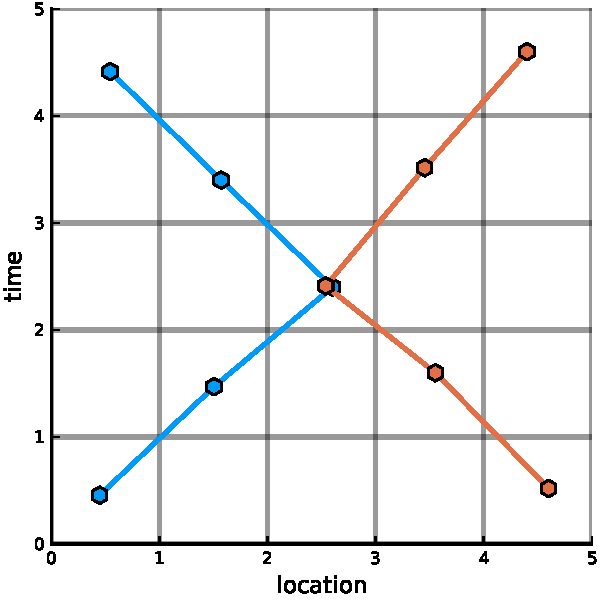
\includegraphics[width=\textwidth]{uturn-c.pdf}
      \caption{}
      \label{fig:u-turn-c}
    \end{subfigure}
    \caption{An adversary having access to the graph in (a) knows that
      the original co-trajectory was either the one in (b) or the one
      in (c). The co-trajectory in (b) seems more likely since it
      corresponds to the two trajectories continuing on their current
      path, whereas (c) would mean that they both perform a U-turn at
      the same time.}
    \label{fig:u-turn}
\end{figure}

We now look at some examples. The first example is an example
co-trajectory which we use to exemplify the above discussion, we look
at a few different kinds of predicates and how they behave with
respect to SwapMob. The second example uses a real world dataset,
T-drive, from taxis in Beijing
\cite{yuan_t-drive:_2010,yuan_driving_2011} and gives an idea of how
SwapMob might perform on real data.

\paragraph{Example co-trajectory}
The co-trajectory \(\cotraj\) used in this part is the one given in
Figure \ref{fig:graph-swap-big-example-orig}. The co-trajectory
consists of five trajectories all consisting of 12 datapoints, it has
six places where a swap can occur and in Figure
\ref{fig:graph-swap-big-example-swap} one possible outcome of applying
SwapMob to it is shown. In Figure \ref{fig:graph-swap-big-example-DAG}
the graph representation \(\swapgraph(\cotraj\) is shown, the
locations of the six swaps are clear. Let \(\paths\) denote the set of
trajectories corresponding to paths in the graph, the number of such
trajectories can be checked to be 49.

\begin{figure}
  \centering
  \begin{subfigure}[t]{0.49\textwidth}
    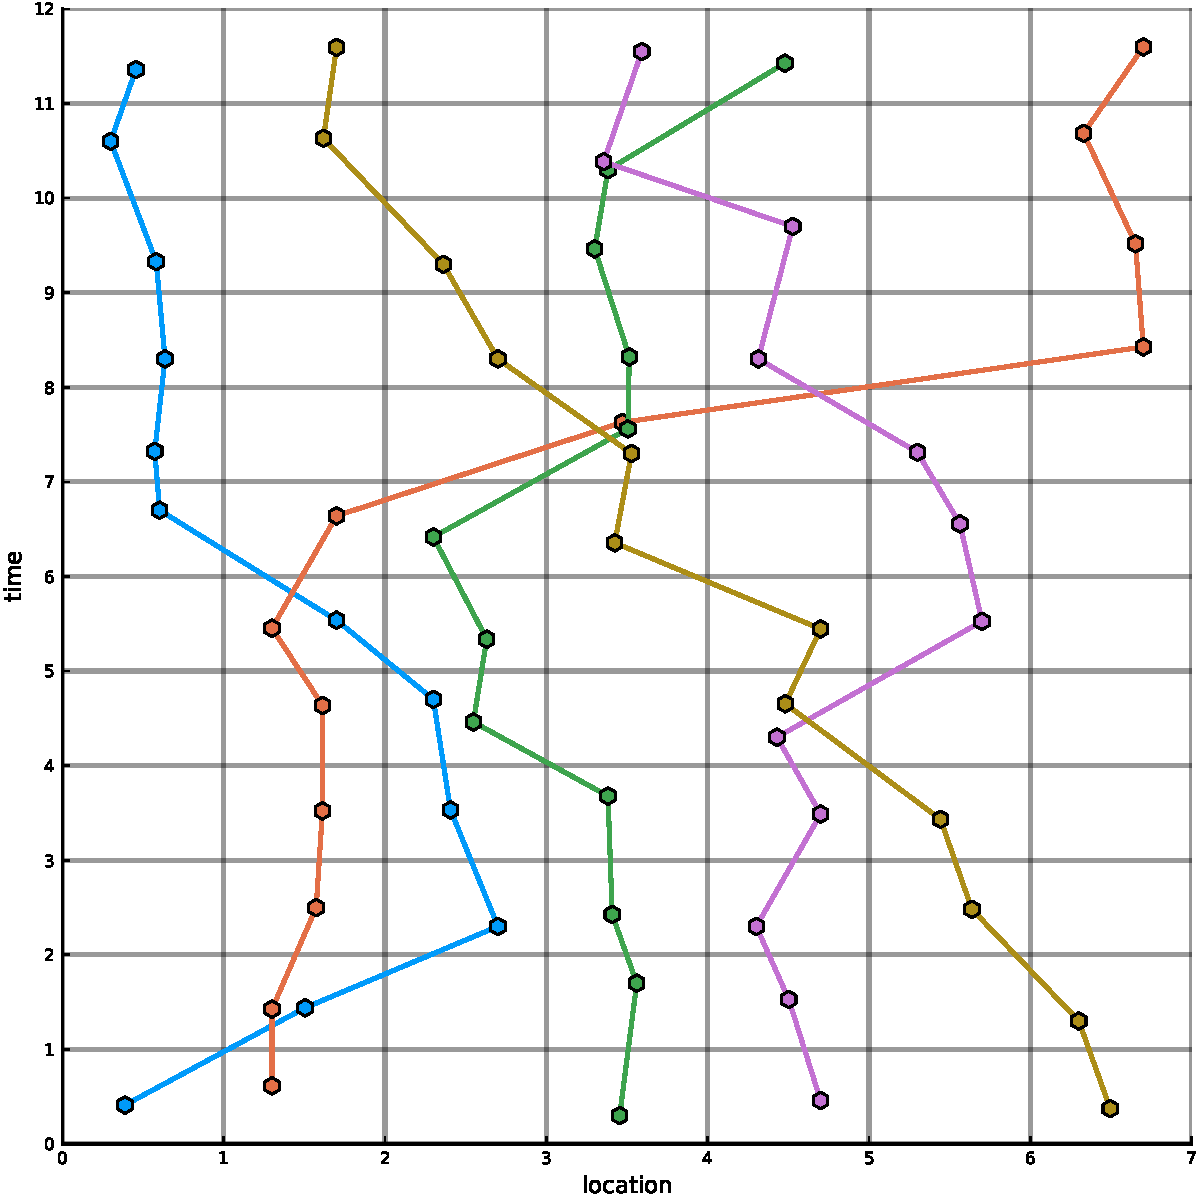
\includegraphics[width=\textwidth]{cotrajectory_example-a.pdf}
    \caption{Original co-trajectory}
    \label{fig:graph-swap-big-example-orig}
  \end{subfigure}
  \begin{subfigure}[t]{0.49\textwidth}
    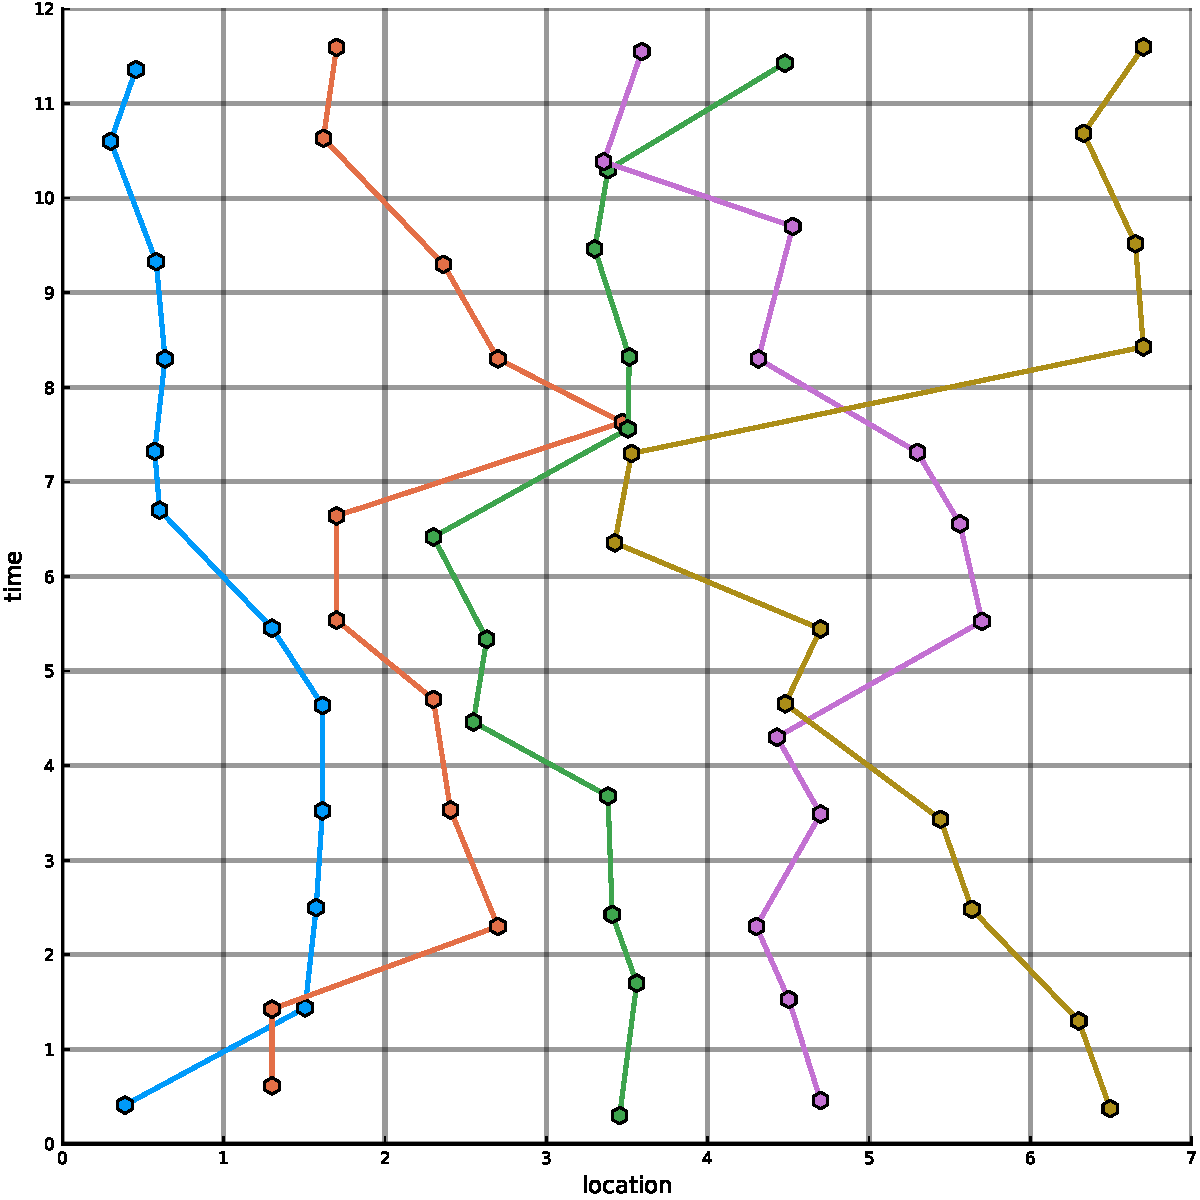
\includegraphics[width=\textwidth]{cotrajectory_example-b.pdf}
    \caption{One possible co-trajectory after applying SwapMob.}
    \label{fig:graph-swap-big-example-swap}
  \end{subfigure}
  \caption{}
  \label{fig:graph-swap-big-example}
\end{figure}

\begin{figure}
  \centering
  \begin{subfigure}[t]{0.49\textwidth}
    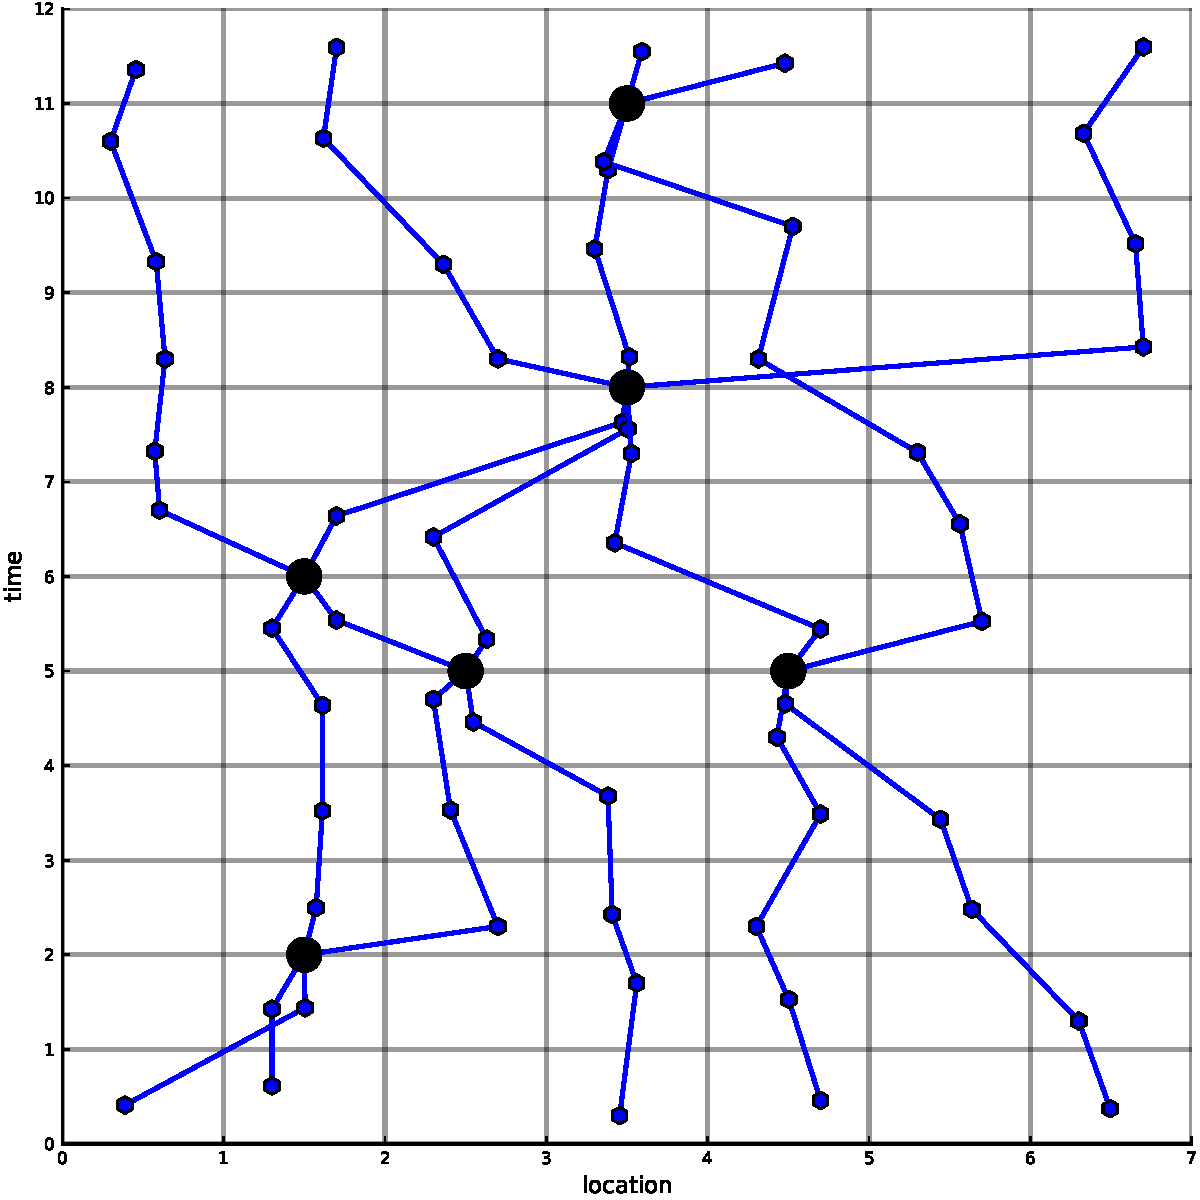
\includegraphics[width=\textwidth]{cotrajectory_example-c.pdf}
    \caption{Representation of the co-trajectory from Figure
      \ref{fig:graph-swap-big-example-orig} as a DAG.}
    \label{fig:graph-swap-big-example-DAG}
  \end{subfigure}
  \begin{subfigure}[t]{0.49\textwidth}
    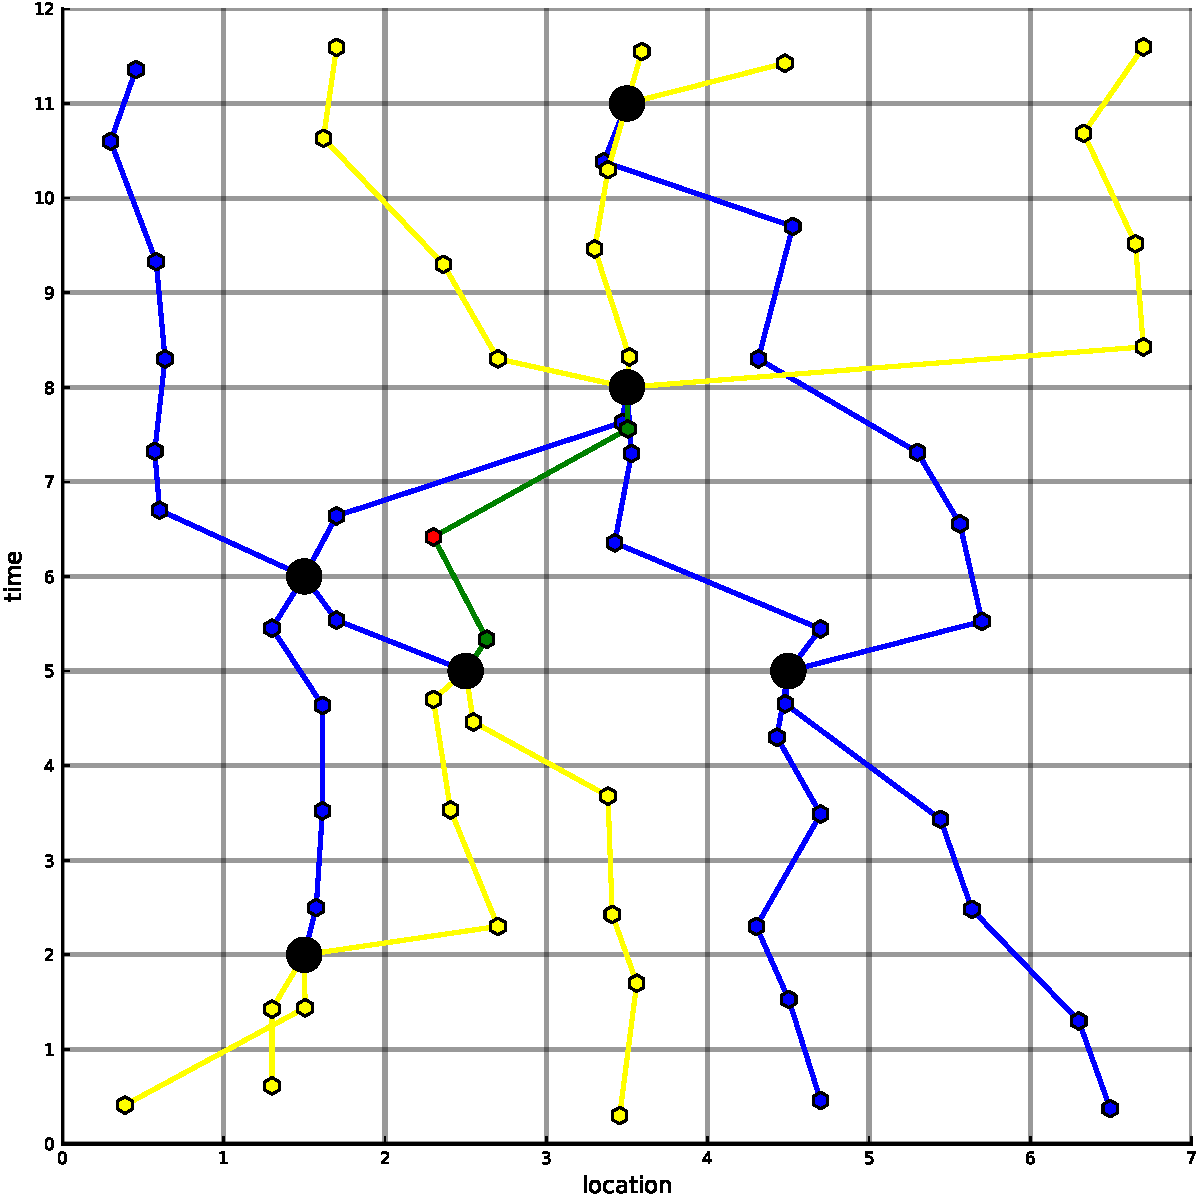
\includegraphics[width=\textwidth]{cotrajectory_example-d.pdf}
    \caption{One datapoint \(\data\) is marked in red. The yellow and
      green lines marks all trajectories having \(\data\) as a
      datapoint. The green part corresponds to datapoints which are
      common for all those trajectories whereas the yellow part
      corresponds to datapoints which are included in only some of
      them. In total there are 12 different trajectories passing
      through \(\data\).}
    \label{fig:graph-swap-big-example-marked}
  \end{subfigure}
  \caption{}
\end{figure}

We begin by considering predicates given by knowing one datapoint of
the trajectory exactly. Assuming we know the datapoint \(\data\) this
gives us the predicate \(\pred_{\data}\) which is true for
trajectories \(\traj\) satisfying \(\data \in \traj\) and false
otherwise. Applying \(\pred_{\data}\) to \(\cotraj\), directly gives
us the trajectory that \(\data\) belongs to since for this
co-trajectory no trajectories have any identical datapoints. If we
instead only have access to the swapped data we have to apply it not
to \(\cotraj\) but to \(\paths\). In this case
\(\pred_{\data}(\paths)\) will not be unique but give us all
trajectories that pass through the given datapoint. For example if
\(\data\) is the datapoint marked in red in Figure
\ref{fig:graph-swap-big-example-marked}, then
\(\pred_{\data}(\paths)\) includes 12 trajectories, marked by yellow
in Figure \ref{fig:graph-swap-big-example-marked}. For this example
SwapMob does increase the privacy since \(\pred_{\data}(\paths)\)
contains many more trajectories than \(\pred_{\data}(\cotraj)\) and we
do not learn exact trajectory of the individual. In terms of
\(k\)-anonymity we have that the co-trajectory satisfies
\(k\)-anonymity with respect to the predicate \(\pred_{\data}\) with
\(k = 12\).

While the privacy in terms of \(k\)-anonymity might be good the
diversity of the set \(\pred_{\data}(\paths)\) is not as high. Some
datapoints are shared by all trajectories in
\(\pred_{\data}(\paths)\) (marked green in Figure
\ref{fig:graph-swap-big-example-marked}) and we therefore know for
sure that the individual has these datapoints in its trajectory. If
we only consider what the trajectory looks like after the datapoint
\(\data\) then there are only four different possibilities, if we care
only about the part before there are three. All of this shows that
while \(\pred_{\data}(\paths)\) does contain many trajectories the
diversity of the trajectories is not as high.

We can also look at the family of predicates given by knowing one
datapoint exactly, i.e. the family of predicates
\(\{\pred_{\data}\}_{\data \in M}\), where \(M\) is the set of all
datapoints occurring in the co-trajectory and \(\pred_{\data}\) is
defined as above. In Figure \ref{fig:paths-dist} the distribution of
\(|\pred_{\data}(\paths)|\) for \(\data \in M\) is shown. We see that
this family of predicates satisfy \(k\)-anonymity with \(k = 4\).

\begin{figure}
  \centering
  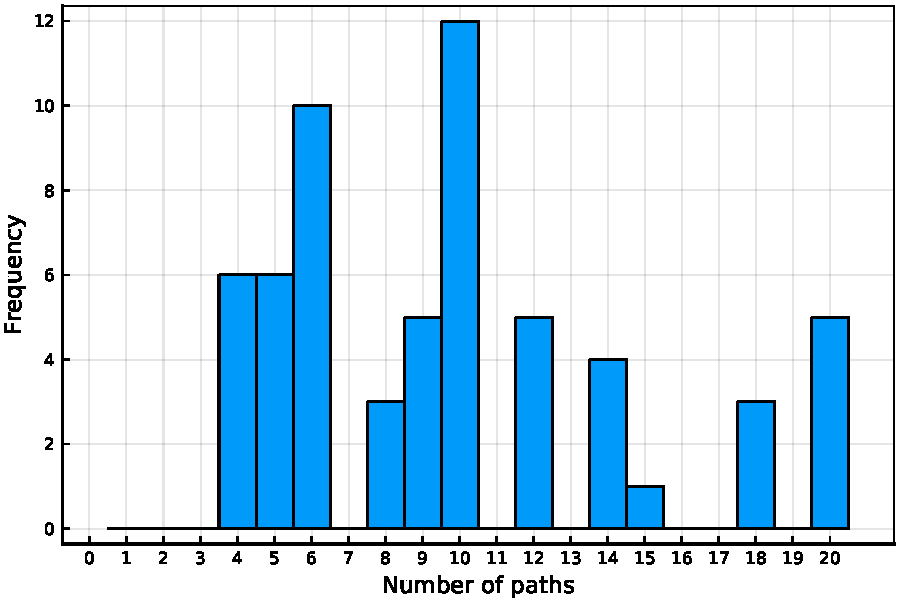
\includegraphics[width=0.5\textwidth]{figures/numpaths_measurements.pdf}
  \caption{Frequency histogram of \(|\pred_{\data}(\paths)|\) for all
    datapoints in the \(\cotraj\).}
  \label{fig:paths-dist}
\end{figure}

Next we consider predicates given by knowing the first and last
datapoint of the individuals trajectory, this gives five predicates,
\(\pred_{1}, \pred_{2}, \dots, \pred_{5}\), each corresponding to one
of the original trajectories. Again we have that
\(\pred_{i}(\cotraj)\) contains the unique trajectory for all
\(1 \leq i \leq 5\). For \(\pred_{i}(\paths)\) we get
\begin{equation*}
  |\pred_{1}(\paths)| = 2,\
  |\pred_{2}(\paths)| = 3,\
  |\pred_{3}(\paths)| = 2,\
  |\pred_{4}(\paths)| = 2 \text{ and }
  |\pred_{5}(\paths)| = 1.
\end{equation*}
Here the privacy gain in terms of \(k\)-anonymity is worse, for this
family of predicates it does not even satisfy \(k\)-anonymity with
\(k = 2\). The diversity is also low, for \(\pred_{1}\) where the
\(k\)-anonymity is the highest all three trajectories in
\(\pred_{1}(\paths)\) are very similar.

\paragraph{T-drive co-trajectory}
The co-trajectory used in this part is based on data from the T-drive
dataset \cite{yuan_driving_2011, yuan_t-drive:_2010}. The dataset
contains GPS trajectories of 10,357 taxis during the period February 2
to February 8, 2008 in Beijing and consists of about 15 million
datapoints.

The datapoints are given by a time together with a position measured
in longitude and latitude. The original data is not clean and does for
example contain many datapoints for which the longitude and latitude
is equal to zero. Therefore we begin by pre-processing the data to
remove these sort of anomalies. To begin with we keep only datapoints
for which the longitude and latitude is inside the box
\([115, 117] \times [39, 41]\), any point outside this box is
definitely outside of Beijing. In addition we discard trajectories
with fewer than 10 datapoints. This gives us a co-trajectory
consisting of 9926 trajectories and a total of 15,650,074 datapoints.

For choosing the partitioning to use with SwapMob the sampling rate
has to be taken into account to avoid problems like those in Figure
\ref{fig:jumps}. The average sampling interval for the trajectories is
about 180 seconds, based on this we choose to partition the time into
intervals of 60 seconds. The average distance between to consecutive
points is about 620 meters, a partitioning into a grid of width 100
meters should then be reasonable. The location is however not given in
terms of meters but in longitude and latitude. In Beijing 100 meters
corresponds to about 0.001 degrees and we can use that for
partitioning. It should be noted that since the earth is a sphere a
uniform grid in terms of longitude and latitude does not correspond to
a uniform grid on the sphere, in our case the precise partitioning is
not important and a uniform grid in longitude and latitude works well.

With the above partitioning the number of possible swaps, as returned
by Algorithm \ref{alg:group-trajectories}, is 540,812. The average
number of swaps for each trajectory is 119 and the distribution of
swaps is seen in Figure \ref{fig:numswaps-a}. Most trajectories
participate in less than 500 swaps but a few participate in thousands.
Of the 471 trajectories that participate in less than 20 swaps the
distribution is seen in Figure \ref{fig:numswaps-b}, 66 of them do not
participate in any swap.

\begin{figure}
  \centering
  \begin{subfigure}[t]{0.49\textwidth}
    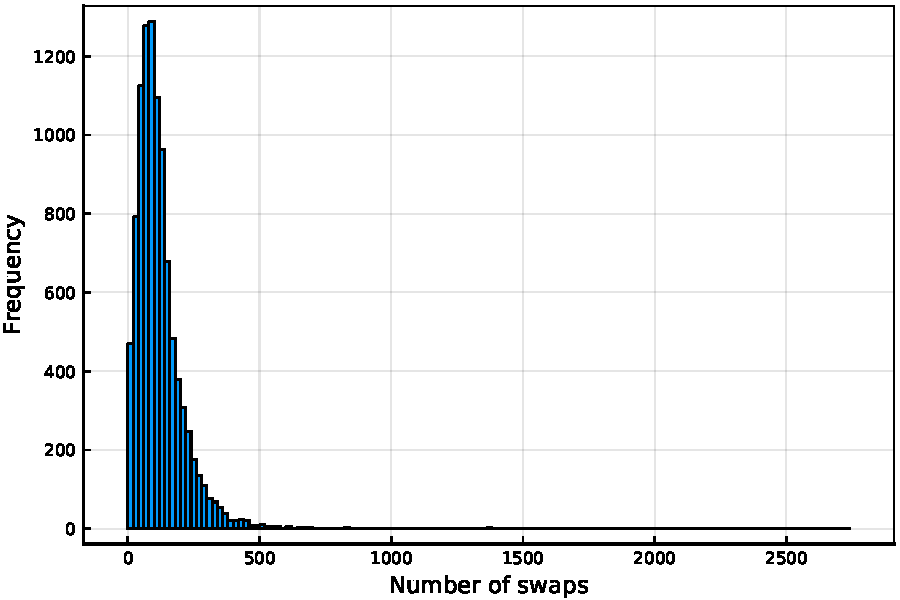
\includegraphics[width=\textwidth]{figures/numswaps-a.pdf}
    \caption{Frequency histogram of number of swaps for all the
      trajectories in the T-drive co-trajectory. The bars in the
      figure has a width of 20.}
    \label{fig:numswaps-a}
  \end{subfigure}
  \begin{subfigure}[t]{0.49\textwidth}
    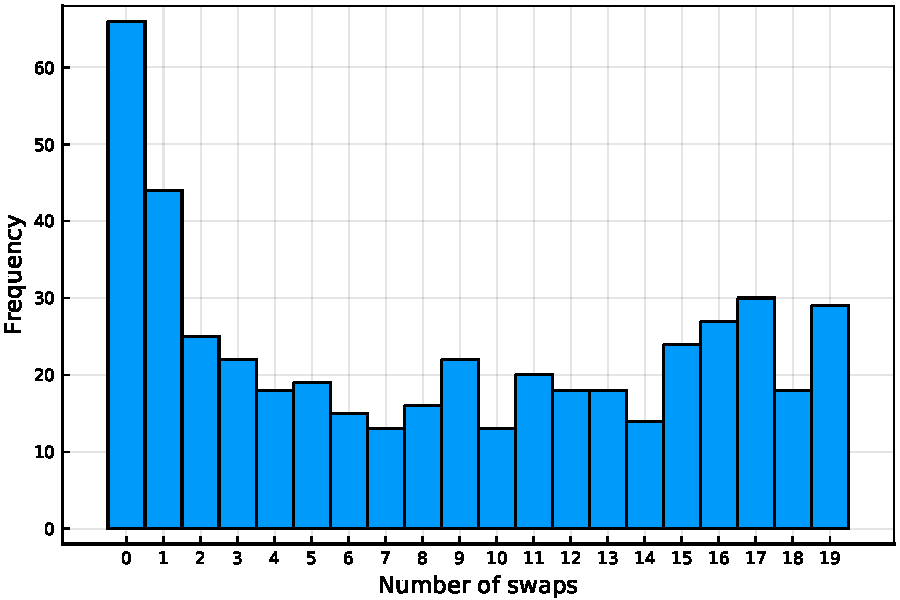
\includegraphics[width=\textwidth]{figures/numswaps-b.pdf}
    \caption{Frequency histogram of number of swaps for all the 471
      trajectories participating in less than 20 swaps. Of these 66
      are seen to not participate in any swap.}
    \label{fig:numswaps-b}
  \end{subfigure}
  \label{fig:numswaps}
\end{figure}

The corresponding graph, \(swapgraph\), is very big and computing the
total number of possible paths gives a result slightly greater than
\(6.7 \cdot 10^{1491}\). From this we can conclude that a naïve brute
force approach for computing \(\pred(\paths\) for a predicate
\(\pred\) would not be feasible, iterating through all possible paths
and checking the predicate is not possible. We therefore have to
restrict our attention to predicates for which \(\pred(\paths)\), or
at least \(|\pred(\paths)|\), can be computed in an efficient way.

Similar to the last example we begin by considering predicates given
by knowing one datapoint of a trajectory exactly. Assuming we know the
datapoint \(\data\) we get the predicate \(\pred_{\data}\). With more
than 15 million datapoints in total we are not able to compute
\(|\pred_{\data}(\paths)|\) for every \(\data\) in the co-trajectory,
instead we take a random sample of around 5\%, about 780,000, of the
datapoints and compute it for these. The result ranges from 1, for
trajectories with no swaps, to around \(10^{2928}\). The cumulative
distribution of \(\log_{10}(|\pred_{\data}(\paths)|)\) is shown in
Figure \ref{fig:numpaths-measurements-cumulative}. As seen in the
figure the \(k\)-anonymity is very big for the vast majority of
datapoints, only 1884 datapoints in the sample have a \(k\)-anonymity
less than \(10^{100}\).

Next We consider predicates given by knowing the first and last
datapoint of the individuals trajectory, this gives 9926 predicates,
\(\pred_{1}, \dots, \pred_{9926}\), each corresponding to one of the
trajectories. In this case we are able to compute
\(|\pred_{i}(\paths)|\) for all \(i\)'s and the cumulative
distribution is given in Figure
\ref{fig:numpaths-startend-cumulative}. For 135 trajectories it is
equal to 1, which means that they are uniquely identified by the
predicate, however it is only for slightly more, 179, trajectories
that it is less than \(10^{100}\).

\begin{figure}
  \centering
  \begin{subfigure}[t]{0.49\textwidth}
    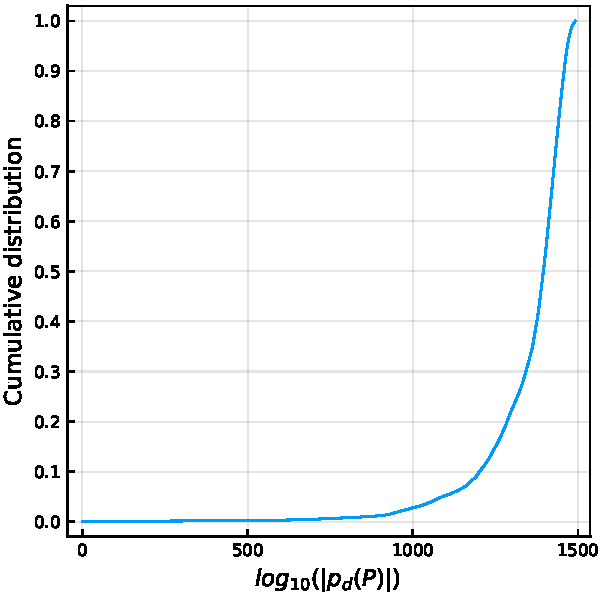
\includegraphics[width=\textwidth]{figures/numpaths_measurements_cumulative.pdf}
    \caption{Empirical cumulative distribution function for a sample
      of \(|\pred_{\data}(\paths)|\) with 5\% of the datapoints.}
    \label{fig:numpaths-measurements-cumulative}
  \end{subfigure}
  \begin{subfigure}[t]{0.49\textwidth}
    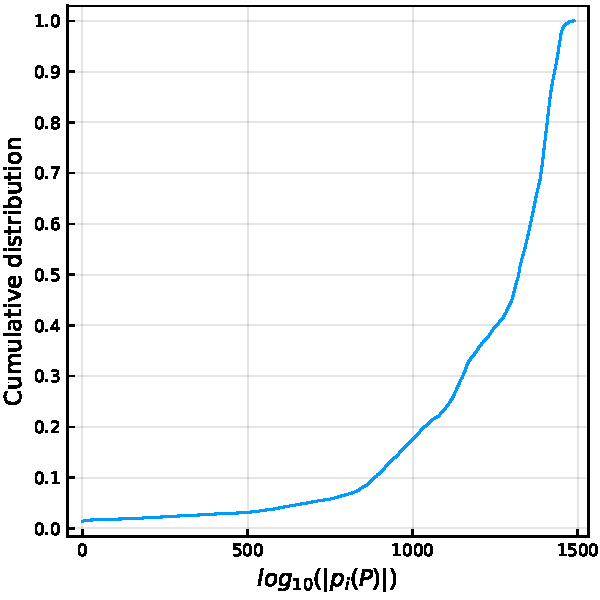
\includegraphics[width=\textwidth]{figures/numpaths_startend_cumulative.pdf}
    \caption{Empirical cumulative distribution function for
      \(|\pred_{i}(\paths)|\) for all trajectories \(\traj_{i}\) in
      the co-trajectory.}
    \label{fig:numpaths-startend-cumulative}
  \end{subfigure}
  \label{fig:numpaths-cumulative}
\end{figure}

We can also make a comparison to the results of de Montjoye et al.
showing that given data about location of mobile phones, as determined
by the carrier's antenna, four datapoints is enough to uniquely
identify 95\% of people in group of one and a half million
\cite{de_montjoye_unique_2013}. Their case is very different from ours
in that the datapoints are not unique, many people are connected to
the same antenna at a time and knowing a datapoint does therefore not
uniquely identify a person. In our case the datapoints are in practice
unique and knowing only one datapoint is enough to uniquely identify
an individual in the original co-trajectory. However, after applying
SwapMob this is, as we have seen, no longer the case and to compare to
de Montjoye et al. we can consider the family of predicates given by
knowing four datapoints of a trajectory. How much protection does
SwapMob give in this case? Given four datapoints,
\(\data_{1}, \data_{2}, \data_{3}, \data_{4}\), we get a predicate
\(\pred_{\data_{1}\data_{2}\data_{3}\data_{4}}\) which is satisfied
for trajectories which contain all four datapoints. Again we are not
able to compute this for all predicates in this family but randomly
sample around 20,000 predicates from the family and compute the number
of trajectories in
\(\pred_{\data_{1}\data_{2}\data_{3}\data_{4}}(\paths)\) for each one.
The sampling is done by choosing first choosing trajectory uniformly
at random and then choosing four distinct datapoints for this
trajectory. The cumulative distribution is given in Figure
\ref{fig:paths-cumulative-3}. The values are in general lower than
those for \(\pred_{d}\)), which is to be expected since four
datapoints conceal more information than one, but similar to those of
\(\pred_{i}\)).

\begin{figure}
  \centering
  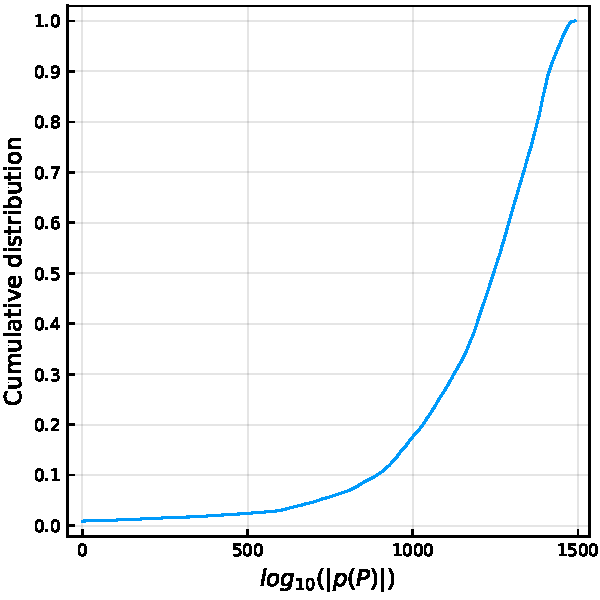
\includegraphics[width=0.5\textwidth]{figures/numpaths_nmeasurements_cumulative.pdf}
  \caption{Empirical cumulative distribution function for
    \(|\pred_{\data_{1}\data_{2}\data_{3}\data_{4}}(\paths)|\) given
    by a sample of size about 20,000.}
  \label{fig:numpahts-nmeasurements-cumulative}
\end{figure}

\subsection{Utility of data}
\label{sec:utility-data}
SwapMob is a tool for improving privacy when working with
co-trajectories. However, to be a useful tool it should not only
improve the privacy but also leave enough structure so that the result
is still useful for analysis. The utility of the data given by SwapMob
has to be sufficiently high or SwapMob would never be used. If SwapMob
preserves enough structure depends on the type of structure is
important for the analysis to be performed. In this section we discuss
what type of structure is and is not preserved by SwapMob and also
some possible use cases for it. Most use cases listed here are related
to mobility data for individuals, in particular in traffic.

On a general level SwapMob does not preserve long time behaviour of
individuals since swapping splits up the trajectories into smaller
pieces. This is important for privacy but means that it cannot be used
whenever long term behaviour is analysed. For example it does not
preserve origin and destination pairs nor does it work for finding
recurring behaviour of trajectories. What it does preserve is local
behaviour, everything between two swaps is preserved. It could
therefore be used to estimate flow of traffic or number of
trajectories caught in red lights.

One important property of SwapMob is that is preserves all individual
datapoints. This means it perfectly preserves the density of
trajectories since this is only based on the number of datapoints in
an area. It can therefore be used to locate popular and less popular
areas.

If we consider all the individual transitions of the co-trajectory,
that is all transitions between datapoints done by trajectories, it is
in general not preserved by SwapMob since at the places where the
swaps are performed these transitions are changed. If we only consider
the transitions up to the partitioning used with SwapMob, i.e. we only
care about between which partitions the transition happen, then it is
preserved by SwapMob. This is visualized in Figure
\ref{fig:swapping-tempo-spatial}. This is relevant for the Markov
chain model for co-trajectories discussed in Section
\ref{sec:markov-chain-models}.

\begin{figure}
  \centering
  \begin{subfigure}[t]{0.49\textwidth}
    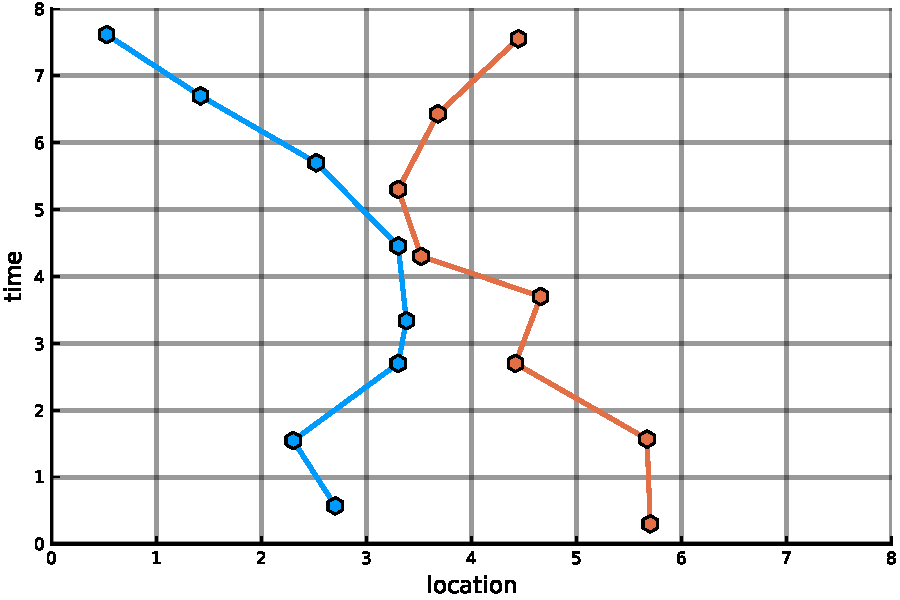
\includegraphics[width=\textwidth]{swapping_tempospatial_grid-a.pdf}
    \caption{Original co-trajectory consisting of two trajectories
      with one possible swap.}
    \label{fig:swapping-tempo-spatial-a}
  \end{subfigure}
  \begin{subfigure}[t]{0.49\textwidth}
    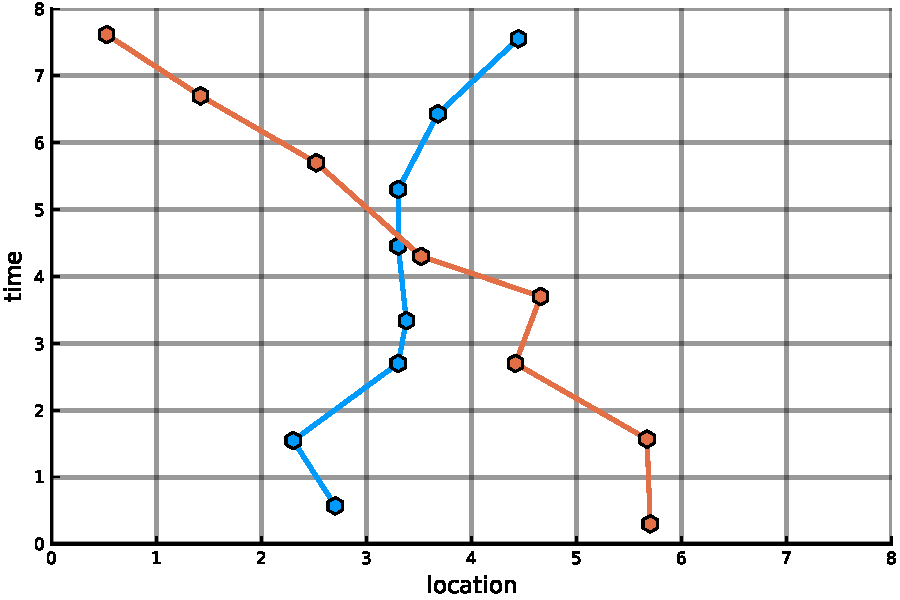
\includegraphics[width=\textwidth]{swapping_tempospatial_grid-b.pdf}
    \caption{Co-trajectory after swapping the two trajectories.}
    \label{fig:swapping-tempo-spatial-b}
  \end{subfigure}
  \caption{Most transitions in (a) are preserved after swapping in
    (b). The only ones that are not are the two transitions between
    the time intervals \([4, 5]\) and \([5, 6]\). If we only consider
    the transitions up to the partitioning of the location space these
    transitions are also preserved, the two transitions changed by
    swapping still correspond to one transition from \([3, 4]\) to
    \([2, 3]\) and one from \([3, 4]\) to \([3, 4]\) in location
    space.}
  \label{fig:swapping-tempo-spatial}
\end{figure}

This is not an exhaustive list of structure that is preserved by
SwapMob. Whenever analysis is performed with data on which SwapMob has
been used care has to be taken to ensure that the conclusion of the
analysis is valid for the original co-trajectory and not only the
co-trajectory resulting from SwapMob.

\section{Modelling co-trajectories}
\label{sec:modell-co-traj}
In this section we discuss different stochastic models for
trajectories and co-trajectories. Stochastic models can be an
important tool when analysing co-trajectories, extracting information
and using it for predictions. For example Markov chain models of
trajectories can be used for next-place predictions
\cite{gambs_show_2010, gambs_next_2012, yan_semitri:_2011}.

We begin by introducing a very general stochastic model for
co-trajectories that is closely related to the definitions of
trajectories and co-trajectories from Section
\ref{sec:traj-and-co-traj}. This model can been seen as a basis on
which more specific models can be built, as an example we define a
Markov chain model for co-trajectories in Section
\ref{sec:markov-chain-models}.

Similar to how a co-trajectory in Section \ref{sec:traj-and-co-traj}
is defined as a collection of trajectories, a stochastic model of a
co-trajectory will be given by a collection of stochastic variables,
each corresponding to a trajectory. In general the location space,
\(\locset\), in which the movement of the trajectories take place can
be any set, however, for simplicity, we assume throughout this section
that the location space is finite. In practice this is not limiting
since most trajectories are bounded in space and we can get a finite
representation by choosing a sufficiently fine discretization. For
example \(\locset\) could be given by a fine grid on a map or a graph
where the nodes represents possible locations.

A trajectory is modelled by a continuous-time stochastic process
\begin{equation*}
  (X_{t})_{t \geq 0} = (X_{t}: 0 \leq t < \infty)
\end{equation*}
with random variables \(X_{t}: \Omega \to \locset\). The location of
the trajectory at time \(t\) is given by the random variable
\(X_{t}\). This model is a bit to general to work well with Definition
\ref{def:trajectory} for trajectories as it allows for trajectories
that cannot be represented in that form. For example it allows for
trajectories which jump to a location, stay there for zero time, and
then jump to another location, something we cannot represent using
Definition \ref{def:trajectory}.

To handle this problem we shall restrict our attention to stochastic
processes that are \emph{right continuous}. In this context, with a
finite state space, a stochastic process \((X_{t})_{t \geq 0}\) is
called \emph{right continuous} if it satisfy that for all
\(\omega \in \Omega\) and \(t \geq 0\) there exists
\(\epsilon \geq 0\) such that
\begin{equation*}
  X_{s}(\omega) = X_{t}(\omega) \text{ for } t \leq s \leq t + \epsilon.
\end{equation*}
Every path \(t \to X_{t}(\omega)\) of a right continuous process must
remain constant for a while in each new state it enters before jumping
to the next state. Restricting to right continuous processes turns out
to be almost enough to be enough to be able to related the model to
Definition \ref{def:trajectory} by considering the \emph{jump times}
and the \emph{jump process} of \((X_{t})_{t \geq 0}\).

The \emph{jump times}, \(J_{0}, J_{1}, \dots\), of
\((X_{t})_{t \geq 0}\), are defined by
\begin{equation*}
  J_{0} = 0,\ J_{n + 1} = \inf\{t \geq J_{n}: X_{t} \not= X_{J_{n}}\}
\end{equation*}
for \(n = 0, 1, \dots\), where \(\inf\emptyset = \infty\). From right
continuity we get that \(J_{n + 1} > J_{n}\) for all \(n\). The
\emph{jump process} of \((X_{t})_{t \geq 0}\) is then the discrete
time process \((Y_{n})_{n > 0}\) given by \(Y_{n} = X_{J_{n}}\).

From here we get a clear relation to Definition \ref{def:datapoint}
of a datapoint, where for \(\omega \in \Omega\) the pair
\((Y_{n}(\omega), J_{n}(\omega))\) gives a datapoint and
\((Y_{n}, J_{n})\) can be seen as a random datapoint with \(Y_{n}\)
corresponding to the location and \(J_{n}\) to the time of the
datapoint. For the set
\(\{(Y_{n}(\omega), J_{n}(\omega))\}_{n > 0}\) to correspond to a
random trajectory according to Definition \ref{def:trajectory} we need
that no two datapoints have the same time, which is true since
\(J_{n + 1} > J_{n}\), and that we have only a finite number of
datapoints in every finite time interval. This last requirement does
not necessarily hold, we have three different possibilities for the
process:
\begin{enumerate}
\item It jumps finitely many times, in which case there is an \(n\)
  such that \(J_{n} = \infty\).
\item It jumps infinitely many times but only a finite number of times
  in every finite interval \([0, t]\), in which case
  \(J_{n} < \infty\) for all \(n\) but
  \(\lim_{n \to \infty} J_{n} = \infty\).
\item It jumps infinitely many times in a finite interval, in which
  case \(\lim_{n \to \infty} J_{n} = \zeta < \infty\).
\end{enumerate}
In the last case the process is said to \emph{explode} and \(\zeta\)
is the \emph{explosion time}. For a trajectory an explosion would
correspond to an infinite number of datapoints in a finite time.
Since we avoided this in Definition \ref{def:trajectory} we choose to
avoid it here as well and therefore further limit the study to
non-exploding stochastic processes.

So by limiting us to right continuous, non-exploding stochastic
processes \((X_{t})_{t \geq 0}\) we can define the discrete stochastic
process \(\{(Y_{n}, J_{n})\}_{n \geq 0}\), which for
\(\omega \in \Omega\) gives us a trajectory
\(\{(Y_{n}(\omega), J_{n}(\omega))\}_{n \geq 0}\) according to
Definition \ref{def:trajectory}. From the definition of \(Y_{n}\) we
have that such a trajectory will never have two datapoints in a row
with the same location, this is different from a general trajectory
where we do allow for multiple consecutive datapoints with the same
location. A general trajectory can be seen as a sampling of a
stochastic process \((X_{t})_{t \geq 0}\) at the times for the
datapoints, then it is possible to have several consecutive samples
where \((X_{t})_{t \geq 0}\) is constant. In this case it is also
possible to miss locations that \((X_{t})_{t \geq 0}\) visits if the
process jumps more than once in between two samples. For any
trajectory \(\traj\) we can get the corresponding jump process and
jump times by removing any consecutive datapoints with the same
location, only keeping the first one.

A co-trajectory can then be modelled by a collection of stochastic
processes \(\{(X_{t}^{i})_{t \geq 0}\}_{i = 1}^{N}\), where the
location of trajectory \(i\) at time \(t\) is given by the random
variable \(X_{t}^{i}\). We here make no assumptions about the
dependencies between the stochastic processes
\((X_{t}^{i})_{t \geq 0}\) and do allow them to be both dependent and
independent of each other.

A natural limitation to put on the processes for the trajectories is
to not allow them to jump from any state in \(\locset\) to any other
state, instead they are only allowed to jump to ``nearby'' states.
What indicates a nearby state depends highly on \(\locset\). If
\(\locset\) is given by the vertices in a road network represented by
a directed graph then it would be natural to only allow movement along
edges of the graph, so if \(Y_{n} = v\) for some vertex \(v\) in the
graph then \(Y_{n + 1}\) must be some vertex to which \(v\) has an
outgoing edge. In general, any limitations on between which states a
process can jump can be modelled by a directed graph with the vertices
given by \(\locset\) and the edges representing allowed jumps.

\subsection{Markov chain models for co-trajectories}
\label{sec:markov-chain-models}
One of the simplest models for a continuous-time stochastic process is
a continuous-time Markov chain model. Essentially, a Markov chain
model for a trajectory is a model where the future movement of the
trajectory only depends on the current location of the trajectory and
not on which locations have been visited before that.

We here give a very brief introduction and definition of a
continuous-time Markov chain and also some notes about how to infer
the Markov structure using data from a co-trajectory. We discuss some
of the benefits and some of the drawbacks of using a Markov chain
model and also mention some possible generalizations of it.

For a complete introduction to Markov chains see any book in the
subject, e.g. \cite{norris_markov_1997}. The introduction we give here
is based on the structure of the \emph{jump times},
\((J_{n})_{n > 0}\) and the \emph{jump process}, \((Y_{n})_{n > 0}\).
From the jump times we can define the holding times
\((S_{n})_{n > 1}\) given by
\begin{equation*}
  S_{n} = J_{n} - J_{n - 1}.
\end{equation*}
They give the time that the process \((X_{t})_{t \geq 0}\) stays in a
state before jumping to the next one. For a Markov chain we should
have that conditional on \(Y_{0} = x_{0},\dots, Y_{n - 1} = x_{n-1}\),
the holding times \(S_{1},\dots, S_{n}\) are independent exponential
random variables of parameters \(q_{x_{0}},\dots, q_{x_{n-1}}\). So
when the process comes to a state \(x\) it stays there for and
exponential time of parameter \(q_{x}\), independent of what has
happened before, after which it jumps to a new state.

For the jump process \((Y_{n})_{n > 0}\) the requirement is that it
should be a discrete time Markov chain. A discrete time Markov chain
is defined by its initial distribution \(\lambda\) that gives the
distribution of \(Y_{0}\) and stochastic matrix \(\Pi\) on \(\locset\)
which gives the probabilities of jumping between two states. A
stochastic matrix on \(\locset\) is given by
\(\Pi = (\pi_{xy}: x,y \in \locset)\) satisfying
\begin{enumerate}
\item \(0 \leq \pi_{xy} \leq 1\) for all \(x, y \in \locset\);
\item \(\sum_{y \in \locset} \pi_{xy} = 1\) for all \(x \in \locset\).
\end{enumerate}
Where \(\pi_{xy}\) is the probability of jumping to state \(y\) from
state \(x\). For it to work properly with the continuous-time Markov
chain we also need that \(\pi_{xx} = 0\) if \(q_{x} \not= 0\), if
\(q_{x} = 0\) then \(\pi_{xy} = 0\) for \(x \not= y\) and
\(\pi_{xx} = 1\). The interpretation of the last part is that if
\(q_{x} = 0\) then the process \((X_{t})_{t \geq 0}\) will never leave
the state \(x\) and the jump process \((Y_{n})_{n > 0}\) will thus
have a zero probability to go anywhere else and probability one to
stay.

To summarize, a continuous-time Markov chain is defined by the triple
\((\{q_{x}\}_{x \in \locset}, \lambda, \Pi)\), where
\(\{q_{x}\}_{x \in \locset}\) determines how long the process stays in
the different states, \(\lambda\) gives the initial distribution and
\(\Pi\) gives the probabilities for jumping between the states.

The simplest Markov chain model for co-trajectories is given by a
collection of trajectories \(\{(X_{t}^{i})_{t \geq 0}\}_{i = 1}^{N}\),
where the trajectories are all independent and identically distributed
continuous-time Markov chains. Since the trajectories are identically
distributed they share the same parameters
\(\{q_{x}\}_{x \in \locset}\) and matrix \(\Pi\).

Using collected data for a co-trajectory the parameters
\(\{q_{x}\}_{x \in \locset}\) and \(\Pi\)) can be estimated. Every
trajectory is then seen as one instance of the Markov chain model and
by removing consecutive datapoints with the same location, only
keeping the first one, we get an instance of the jump process and the
jump times for every trajectory. With this, the parameters
\(\{q_{x}\}_{x \in \locset}\) can be estimated by the average holding
times for the different states, i.e. \(q_{x}\) is given by the average
time a trajectory stays in the state \(x\). The matrix \(\Pi\) can be
estimated by considering the transitions between the states, for a
state \(x\) all transitions going out from that state are collected
and the probabilities \(\pi_{xy}\) are then given by the number of
transitions from \(x\) to \(y\) divided by the total number of
transitions from \(x\).

As mentioned in Section \ref{sec:utility-data} SwapMob preserves
transitions on partitioning used. If the same partitioning is used for
the Markov chain SwapMob will thus preserve the estimate of \(\Pi\)).
The holding times \(\{q_{x}\}_{x \in \locset}\) will also be preserved
when swapping which means that SwapMob fully preserves the estimated
Markov chain.

The Markov chain model gives a very local picture of a co-trajectory.
The transition probabilities gives information about general direction
of movement in a location, where trajectories are most likely to go
directly after visiting it. The parameters
\(\{q_{x}\}_{x \in \locset}\) give information about how long time a
trajectory usually spend at the locations. If the trajectories
represent people this could give information about what type of
activities are carried out at the location, we expect someone to stay
longer at the cinema than at the super market, but if the trajectories
represent vehicles it could be interpreted as speed.

By comparing co-trajectories collected at different times this can
give a quantitative measure of differences. Comparing the holding time
parameters gives us information about changes in how long time
trajectories spend at a location, this could for example indicate
changes in traffic flow. From the transition probabilities we can see
changes in direction of movement, for example by comparing
co-trajectories from the morning with ones from the evening we could
see differences based on the commuting going in different directions.

There is however a lot of information in co-trajectories that the
Markov chain model does not capture, it does not handle global nor
time dependent behaviour well. One example of global behaviour it does
not capture is movement between two locations that are far from each
other. The Markov chain can only capture the individual transitions
between all locations in between but since it only takes into account
the last visited location it cannot track the whole path. Most
movement of people is time dependent, for example during the morning,
the day and the evening the movement is very different. Since the
transition probabilities in the Markov chain does not depend on time
this cannot be taken into account. What can be done is to consider
several different models, using data from the morning to make a model
for the morning, data from the day to make a model for the day and
data from the evening to make a model for the evening. In this way you
can see differences in behaviour by comparing the different models,
however this requires you to manually choose the times for each model.

Another thing this model does not handle is dependencies between
trajectories, in this simple model all trajectories are assumed to be
independent. Often times there will be dependencies between
trajectories, for example in traffic flow trajectories that are close
to each other will have a similar flow.

There are many possible generalizations that can be made to this
simple model. One natural generalization is to let the transition
probabilities depend not only on the current state but on the last
\(n\) states. Another one is to allow different trajectories to be
modelled by different Markov chains. This would make sense if there
are different classes of trajectories, in which case a separate Markov
chain model could be used for every class.

\section{Conclusions and future work}
We have presented a method, SwapMob, for enhancing privacy when
working with co-trajectories. We have given a graph representation of
the method for analysing the increase in privacy that it gives. When
analysing the privacy for a real dataset we have seen that SwapMob
greatly increases the \(k\)-anonymity. SwapMob also preserves many
properties that are important for analysis, such as datapoint density
and local behaviour of trajectories.

The main focus for future work would be to continue to analyse the
privacy given by SwapMob. Considering other measures for privacy than
\(k\)-anonymity, in particular coming up with a way to measure
diversity, would be important. Also considering different kinds of
predicates, with a focus on those that would be likely to encounter in
practice. Taking a look at other kinds of privacy that just
re-identification attacks would also be of interest.

A very general stochastic model for co-trajectories was introduced.
While it could serve as a base for other more specific models it is by
itself most likely to general to be of use. One more specific mode, a
Markov chain model, was defined together with how to estimate its
parameters using data from a co-trajectory. Some generalizations of
the Markov chain model were also discussed.

We have only taken a very brief look at stochastic models for
co-trajectories and there is much potential for future research. It
would be of interest to apply the Markov model to real questions about
real data to see how useful it is. Looking further at possible
generalizations of the Markov model as well as studying other types of
stochastic models is also a line to go.

\bibliographystyle{unsrt}
\bibliography{references.bib}

\end{document}

%%% Local Variables:
%%% mode: latex
%%% TeX-master: t
%%% End:
